\documentclass{class}
\mcmsetup{CTeX = false,
        tcn = 14632, problem = A,
        sheet = true, titleinsheet = false, keywordsinsheet = false,
        titlepage = false, abstract = false}
\setlength{\headheight}{13.6pt}
\usepackage{bookman}
%\usepackage{times}
%to get dummy loremipsum text
\usepackage{lipsum}
\usepackage{subcaption}
\usepackage{booktabs}
\usepackage{minted}
\usepackage{longtable}
\usepackage{amsmath}
\usepackage{mathtools}
\usepackage{blkarray}
\usepackage{caption}
\usepackage{nicematrix}
\usepackage{longtable}
\usepackage{xltabular}
\usepackage{graphicx}
\usepackage{lmodern}
\usepackage{algorithm2e}
\usepackage{titlesec}
\RestyleAlgo{ruled}
\usepackage{pdfpages}
% \usepackage{newpxtext,newpxmath}
\usepackage[numbib,nottoc]{tocbibind}
\usepackage[svgnames]{xcolor}
\usepackage{multicol}
\usepackage[none]{hyphenat}
\usepackage{ragged2e}


%%% BIB SPACING
\usepackage{bibspacing}
\setlength{\bibitemsep}{.2\baselineskip plus .05\baselineskip minus .05\baselineskip}

%for unknown reason, including the following packa4ges changes the style of the contents section
% \usepackage{multicol}
% \usepackage{tocloft}
% \usepackage{titletoc}
\title{HiMCM}

%% CODE FORMATTING COMMAND
\newcommand{\insertcode}[2]{
    % #1 is what filename shows up as
    % #2 is what actual filepath is
    \textcolor[rgb]{0.98,0.00,0.00}{\texttt{\textbf{#1}}}
    \vspace{0.2em}
    \hrule
    \begin{multicols}{2}
    \inputminted[breaklines, linenos, breakanywhere=true, breaksymbolleft=, breaksymbolright=, numbersep=5pt, xleftmargin=\parindent, style=vs, fontsize=\tiny]{python}{#2}
    \end{multicols}
}
%%%%%%%%%%%%%%%%%%%%%%%%%%%%


%% Assumption Table Numbering
\newcounter{assumption}
\newcommand{\nextassumption}{\refstepcounter{assumption}\arabic{assumption}}
%%%%%%%%%%%%%%%%%%

%% SMALL CAPS FONT
\renewcommand{\theFancyVerbLine}{\sffamily\textcolor{gray}{\scriptsize\arabic{FancyVerbLine}\hspace{8pt}}}
%%%%%%%%%%%%%%%%%%%%%%%%%%%%

%%%% CHANGE MARGINS COMMAND %%%%%

\def\changemargin#1#2{\list{}{\rightmargin#2\leftmargin#1}\item[]}
\let\endchangemargin=\endlist 

%%%%%%%%%%


%% TITLE PAGE. SUMMARY PAGE FORMATTING
\titleformat{\section}[block]
{\fontfamily{cmr}\centering\large\scshape\bfseries}{\thesection}{1em}{}
\titlespacing*{\section}
{0pt}{2.5ex plus 1ex minus .2ex}{2.5ex plus .2ex}
\date{\today}
\begin{document}
\begin{abstract}

%%%% SUMMARY PAGE %%%%%
\begin{center}
{\fontfamily{cmr}\large\scshape\bfseries Summary}
\end{center}
\begin{changemargin}{0.3in}{0.3in} 
\textsc{We are here to "spread"} the news about dandelions and their effects on our environment. Problem A consisted of two sub-tasks: (1) modeling the spread of a single dandelion across a one-hectare plot of land over the course of one year and (2) developing a method to measure the impact of a foreign species in a new environment. 
  
To model the spread of dandelions over a plot of land, we developed a \textit{Seed Agent Model}, which follows a dandelion's life cycle from seed to plant to puffball, including germination, growth, and death. We decided to use the Brownian Motion Process to model random dandelion movement and treat seed growth and death as a stochastic agent-based problem, meaning each seed was treated independently. To make our model adaptable to different regions and climates, we introduced several \textit{hyperparameters} of temperature, light, wind, consumers, and soil nutrients, which are calibrated by location.

After we developed our model, we collected easily accessible data for our hyperparameters from three different climate regions: Clay, NY (temperate); Phoenix, AZ (arid); and Florida Keys, FL (tropical). Our results show that dandelion population growth tends to follow a similar cyclical trend year-over-year, where plant populations spike in their seed dispersal and blooming seasons and remain dormant otherwise, regardless of the region's climate; however, different regional climates resulted in different blooming seasons. Across all three regions, our model yielded a final population of around \(500\) to \(900\) dandelion plants after one year. Lastly, to test the validity of our model, we employed a Monte Carlo sampling simulation (\(\pm 10\%\)) and a sensitivity analysis of all hyperparameters, which revealed that light levels and seed lifespans significantly affect dandelion growth, whereas nutrients found in the soil were not as impactful.

For part two, we developed a "trade-off" model that considers both the benefits and disadvantages of introducing a foreign species. This was done by splitting the perceived impact into two components: harmful ecological and beneficial economic impact. Concerning the foreign species' impact on their new environment, we assessed their effect on native species and the speed at which they spread. To do this, we used a Lotka-Volterra system of differential equations and a logistic regression of population data, respectively. As for the economic potential of the foreign species, we conveyed the societal impact as a standardized monetary value. To do so, we used the bioeconomic Gordon-Schaefer model to represent the profit made from the plant and Sen's Welfare functions to calculate the plant's social benefits and human health impact. 

From there, we applied the second model to three foreign species — dandelions, garlic mustard, and English ivy — and compared each plant's results. If the economic benefit was significantly higher than the ecological impact, we denoted the species as "non-invasive;" otherwise, it was labeled "invasive." By comparing each plant's results, we decided dandelions were invasive species due to their high ecological impact and below-par economic benefit. Similarly, garlic mustard plants were also considered as invasive, whereas English ivy was considered non-invasive. A benefit of this model is its generalizability to almost any type of plant due to our proposed \textit{Data-Score-Divide} (DSD) framework. Using this framework, species can be automatically classified as invasive or non-invasive by a user-determined threshold to represent the balance between ecological and economic impact scores. 

Overall, our agent-based and stochastic models thoroughly represent dandelions in the environment, how they spread, and their role as an invasive species. Easily adaptable, our models can be used on virtually any plot of land and for any type of invasive species. Although they seem irrelevant growing in your yard, the effects of dandelions on the environment can "blow" you away. \#dandelionPRIDE

\end{changemargin} 
\end{abstract}
%%%%%%%%%%%%%%%%%%%%%%%%%%%%%%%%%%%%%%%%$

\maketitle

% \centerline{\fontfamily{cmr}\centering\large\scshape\bfseries{Infographic/Letter/Etc}}

% infographic, letter, etc.

% \newpage

%%% TABLE OF CONTENTS %%%%


\begin{changemargin}{0.3in}{0.3in}
{%\baselineskip=20pt
\tableofcontents
}
\end{changemargin}

\setlength{\parskip}{0.05em}

\newpage
\section{Introduction}

\subsection{Background}
Everyone knows the best way to make a wish: picking up a dandelion in its iconic "puffball" stage and blowing on it to release thousands of seeds into the environment. But how much do these seeds contribute to dandelion growth and spread? In this paper, we develop a mathematical model to predict the spread of dandelions across a plot of land and evaluate whether plants like dandelions are truly invasive.

Beginning as one tiny airborne seed, there are several phases that a dandelion progresses through in its lifetime. The first phase is when the seeds of a "puffball" spread, usually by wind. Once landed in soil, the seed will begin its plant phase, which has two main processes: (1) germination, where the seed breaks dormancy, and (2) growth as a plant, where the seed continues to adapt to the environment, eventually becoming the iconic bright yellow flower. Finally, in the third phase, the dandelion flower returns to a puffball stage to disperse even more seeds, thereby restarting the cycle. Although the cycle lasts about 50 days on average, it often resets randomly due to unpredictable variables, such as predator consumption, inclement weather, or a possibly unsuccessful growth stage \cite{stewart-wade_biology_2002}.

\begin{figure}[h!]
\centering
    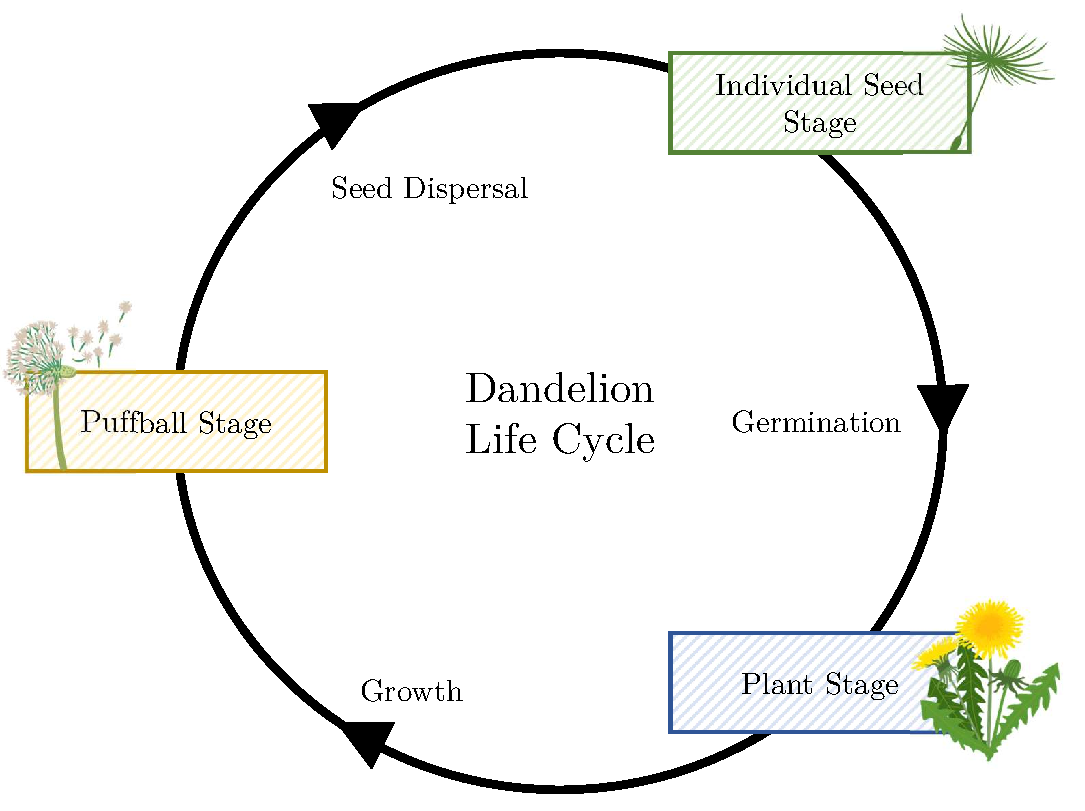
\includegraphics[scale=0.5]{figures/dandelionlifecycle.pdf}
    \captionsetup{width=0.9\textwidth}
    \caption{\textbf{Dandelion life-cycle.} A recurring process from seed to germination to growth, then the dispersal of seeds again.}
    \label{fig:dandelionlifecycle}
\end{figure}

\subsubsection{Phase 1: Seed}
Dandelion seeds begin their dispersal process from a puffball. However, only around 2-4\% of the many seeds make it past the initial dispersal stage, the remainder of which is lost to consumers \cite{noauthor_dandelion_nodate-2}. Upon landing, it will lay dormant until it meets certain environmental conditions to germinate and begin its plant growth process. 

% In order for a seed to grow, certain environmental conditions must be met. In the event that conditions are not met, seeds often enter a dormant stage where they can remain beneath the earth until environmental conditions are met. Unlike most plants, the dandelion seed cannot lay dormant for long due to the high likelihood of premature consumption \cite{noauthor_dandelion_nodate-2} Of the small amount that does survive, they typically germinate right away and survive until the next season \cite{noauthor_dandelion_nodate-2}.

\subsubsection{Phase 2: Plant}
Next, the seed continues into the plant growth process. Here, certain environmental conditions, such as the right temperature, light, and nutrients in the soil can aid the growth of a dandelion. The dandelion is no longer considered growing when it has reached its puffball phase.

\subsubsection{Phase 3: Puffball}
The puffball stage occurs when the white seeds of the plant fully emerge, replacing the distinctive yellow flowers  \cite{board_of_pesticides_control_maine_dacf_dandelion-taraxacum_nodate}. Once ready, the dandelion releases its seeds to the power of the wind which scatters the seeds into an everlasting journey.

\subsubsection{Death}
As a perennial plant, the taproot of the dandelion allows the plant to keep its roots for another year while the flowers and stem wither away in the winter. In the event of any damage to the portion of the plant above ground, the taproot remains rooted, and so, the dandelion continues to survive \cite{farmshowGrowingDandelions}. For a dandelion to die fully, either the taproot is entirely removed from the ground, or the plant reaches its life expectancy of 10-13 years \cite{noauthor_garden_nodate}. In Figure~\ref{fig:dandelionlifecycle}, we summarize the life cycle of a dandelion (from seed to puffball), from which we draw inspiration in our dandelion spread model.

\subsection{Problem Restatement}

 \begin{enumerate}
 \item Develop a model to represent the spread of dandelions over the course of 1, 2, 3, 6 and 12 months, given the model begins with a single dandelion in its puffball stage adjacent to an open, one-hectare plot of land.
\item Formulate a mathematical model to determine an "impact factor" for invasive species.
\subitem a. Compute an impact factor for dandelions to test the model.
\subitem b. Determine the impact factor for two other non-native plant species of 
our choice that are often considered invasive.

\end{enumerate}


%% MODEL 1 %%
\section{Part 1: Modeling the Spread of Dandelions}

\subsection{Problem Analysis}
Because a dandelion is a living organism, its life follows a cycle through the several phases outlined in the previous section and in Figure~\ref{fig:dandelionlifecycle}. In addition to the cyclic nature of dandelion growth, some unpredictability exists due to changing environmental factors such as the wind and consumers. 

% So, we decided to model such factors with randomness because of the unpredictable nature of environmental and growth conditions.

%where the dandelion transforms from seed to puffball, is based on factors that change over time, including temperature, light, and nutrients. Once a dandelion reaches the puffball stage, those released seeds further contribute to the spread of dandelions.

\subsection {Assumptions}

\begin{table}[h]
\renewcommand{\arraystretch}{1.3}
    \begin{tabularx}{\textwidth}{lp{0.3\textwidth}X}
    \toprule
    \textbf{\#} & \textbf{Assumption} & {\centering \textbf{Justification}}  \\ \midrule
    
    \raggedright \nextassumption\label{assumption:1} & Dandelion seeds that land outside of the one-hectare plot of land will not be considered.  & The problem statement refers to a dandelion adjacent to a plot of land, so we interpreted that as modeling the growth of dandelions on that plot of land only. \\

    \rowcolor{gray!15} \raggedright \nextassumption\label{assumption:2} & Dandelion seeds behave mostly independently. & This allows us to develop an agent-based model to analyze each individual seed and easily adjust hyperparameters. \\

    \raggedright \nextassumption\label{assumption:3} & Although consumers are considered on the plot of land, human disturbances do not occur.  & Because information is not provided on the whereabouts of the plot of land, we assume that no humans will cause a significant disturbance to the growth of the dandelions. \\

    \rowcolor{gray!15} \raggedright \nextassumption\label{assumption:4} & No natural disasters will occur during the 12-month period we are modeling.  & Because the probability of a natural disaster occurring is low \cite{botzen_economic_2019}, our model does not consider it. \\

    \raggedright \nextassumption\label{assumption:5} & Nitrogen and potassium are the only nutrients affecting the growth of dandelions. & Higher potassium and nitrogen levels in the soil are the primary factors for increased seed germination and growth speed. \cite{noauthor_dandelion_nodate-2}.\\

    \rowcolor{gray!15} \raggedright \nextassumption\label{assumption:6} & Wind is the only factor that spreads the seeds from a puffball.  & As stated previously, no human disturbances could cause seeds to spread; therefore, wind is the only other natural factor that can affect seed dispersal. \\ 

    \raggedright \nextassumption\label{assumption:7} & Our model begins on January 1st, and ends on December 31st. & To model an entire year and include climate-related factors in our model, we are assuming that the first dandelion of the model exists on January 1st and is modeled until December 31st. \\ 

    \rowcolor{gray!15} \raggedright \nextassumption\label{assumption:8} & The one-hectare plot of land is square (100 meters by 100 meters). & By specifying the dimensions of the plot of land to be a square, we can better model the movement of dandelion seeds. \\ 
    \bottomrule
    
    \end{tabularx}
    
\end{table}

\subsection{Brief Overview}
First, we model the spread of the seeds from an initial puffball across a one-hectare plot of land. Afterward, we minimize the scope of the problem, focusing on each individual seed to model the independent growth of a seed. Once each seed matures into a puffball, the process repeats.

To model the life cycles of a seed, we developed a \textit{Seed Agent Model}, which considers environmental characteristics, such as wind, temperature, sunlight, and nutrients, to iterate each seed through a germination and plant growth life cycle. Finally, when new puffballs are fully developed, the Seed Agent Model is again applied to model the spread and growth of every new seed. Throughout our process, we incorporate environmental unpredictability by developing several stochastic processes. 

Below is a table of variables used throughout our agent-based model.

\begin{table}[h]
\renewcommand{\arraystretch}{1.3}
%p{0.8\linewidth
    \begin{tabularx}{\textwidth}{p{0.2\textwidth} lX}
    \toprule
    \textbf{Variable}           & \textbf{Symbol} & \textbf{Description}  \\ \midrule
    \raggedright Time Step & $t$  & Each time step is a day where \(t = 0\) is January 1 of a year. \\
    \rowcolor{gray!15}
    \raggedright Number of Moves & $N$  & Number of moves a seed takes in movement process. \\
    Coordinate Shift & $\Delta x, \Delta y$    &  Change in \(x\) or \(y\) coordinate of a seed in every move.  \\
    \rowcolor{gray!15} \raggedright  Death Date & $D$               &  Time of death of a seed, sampled from Exponential distribution.  \\
    \raggedright Plant Growth & $G$ & The stage of growth of a dandelion plant between 0 and 1. \\
    \rowcolor{gray!15} \raggedright Temperature Index & $T_I$ & A standardized metric to describe optimal temperatures for dandelions. \\
    \raggedright Light Index & $L_I$ & A standardized metric to describe optimal light levels for dandelions. \\
    \rowcolor{gray!15} \raggedright Nutrition Index & $N_I$ & A standardized metric to describe optimal soil conditions for dandelions. \\
    \bottomrule
    \end{tabularx}
\end{table}

\subsection{The Way Of The Wind: A Seed Dispersal Process}

We first identified the primary contributing factor of dandelion seed movement to be the wind \cite{wang_separating_2021}, following Assumption~\ref{assumption:6}. Thus, we decided to use the Brownian Motion Process to model the spread of dandelion seeds. Brownian Motion stochastic processes are often utilized to model the stochastic, or random, movement of particles in a particular medium, such as seeds in open air.

To begin, we define the number of seeds of the initial puffball dandelion to be \(S_0\). The puffball releases its \(S_0\) seeds into a \textit{stochastic Brownian motion process} in a 2D plane. 

To mimic the random nature of wind in determining a seed's new position, each seed will complete two stages of an algorithm. First, a seed is assigned a random number of position translations, or "moves." Next, the distance the seed moves in that position is randomly determined for each position translation. This allows us to model the varying movements of the dandelion seeds in all directions.

\subsubsection{Number of "Moves" a Seed Performs}
    First, we determine \(N\), the number of "moves" a seed will perform on the 2D plane in time-step \(t\). Next, we use a probabilistic model to account for varying winds in different climates and days. Therefore, we assign the random variable \(N\) with a non-homogeneous (changing over time) Poisson distribution and wind strength hyperparameter \(m(t)\), denoting the mean number of steps at time step \(t\). Poisson probability distributions are used when finding the number of events that occur in a given time frame. We can model this as 

    \begin{align}
        N & \sim \text{Poisson}(m(t)) \\
        \mathbb{P}(N=n) & = e^{-m(t)}\frac{\left[m(t)\right]^2}{n!} \nonumber
    \end{align}

    In other words, the number of moves a seed will take will be sampled from this Poisson distribution, which changes according to wind levels (Note: wind levels change based on the region and time). We use \(k\) to denote the \(k\)'th move out of \(n\) moves such that \(k \in [0, n]\).

\subsubsection{Distance Per "Move"}

    Next, we determine the change in position for each move \(k\). The seed will move a specified distance \(\Delta x\) and \(\Delta y\) which are sampled from a \(\text{Normal} (0, \sigma^2)\) such that the new coordinate for each seed after step \(k\) will be 

    \begin{equation}
        (x_i, y_i)_{k+1} = (x_i, y_i)_k + (\Delta x, \Delta y)
    \end{equation}

    \begin{align}
        \Delta x \text{ or } \Delta y & \sim \text{Normal}(0, \sigma^2) \\
        \mathbb{P}(\Delta x \text{ or } \Delta y = d) & = \frac{1}{\sigma \sqrt{2\pi}}e^{-\frac{1}{2}\left( \frac{d}{\sigma}\right)^2} \nonumber
    \end{align}
    
Recall that from Assumption~\ref{assumption:1}, dandelion seeds that travel outside our provided hectare of land are removed from the consideration of our model to simplify our model's scope.

\subsection{Race the Clock: Beating a Death Date}
After the seed is assigned a new location, the seed will go through two critical processes: (a) germination and (b) plant growth. However, the seed may die of natural causes before each phase. To account for this nuance, we introduce a \textit{Death Date} for each seed that resets at the end of the germination and plant growth stage. 

The first death date of a seed will be assigned after it lands on the ground and before it begins the germination process. The death date is determined by randomly sampling from a probabilistic survivorship curve (see Figure \ref{fig:exponentialdistribution}). If the seed successfully germinates before its assigned death date, it will be assigned a new death date for the plant growth cycle. 

\begin{figure}[h!]
\centering
    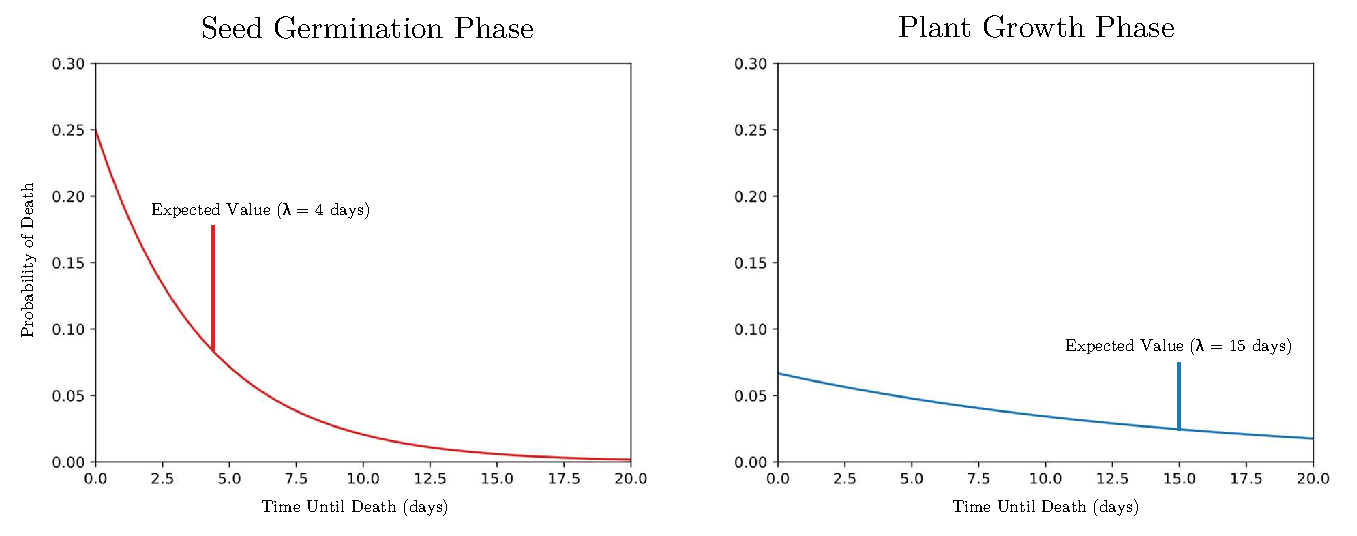
\includegraphics[scale=0.65]{figures/exponentialdistribution.pdf}
    \captionsetup{width=0.9\textwidth}
    \caption{\textbf{The survival rate of a seed during two major phases.}}
    \label{fig:exponentialdistribution}
\end{figure}

The survival rate of dandelions is often classified as a Type III survivorship curve \cite{noauthor_53_nodate}, where shorter lifespans are more probable than longer lifespans. Thus, due to the low percentage of seeds that eventually germinate, it is more likely to randomly select a relatively earlier death date than a later death date \cite{noauthor_dandelion_nodate-2}. 

Henceforth, we used a non-homogeneous (time-varying) Exponential distribution to model survival rates. However, per Assumption~\ref{assumption:2}, the only time dandelions are not independent is when two seeds land in the same place, thereby eliminating one of the two.

The probability of the random variable of seed death date \(D\) at time \(t\), \(\mathbb{P}(D = t)\), can be determined by finding the \textit{survivorship curve} of dandelions in their respective environments. 

\begin{align}
    D & \sim \text{Exponential}(\lambda(t)) \nonumber  \\
    \mathbb{P}(D = t) & = \lambda(t) e^{-\lambda(t) t}
\end{align}

where \(\frac{1}{\lambda(t)}\) is the average lifespan of a dandelion seed at time step \(t\). For regional calibration, \(\lambda(t)\) can be adjusted. For the sake of differentiating the death date of seeds and dandelion plants, we will introduce two hyperparameters \(\lambda_s(t)\) and \(\lambda_d(t)\) for the two stages, respectively \cite{board_of_pesticides_control_maine_dacf_dandelion-taraxacum_nodate}. Note that because no natural disasters nor human disturbances will occur on our hectare plot of land (Assumptions~\ref{assumption:3} and~\ref{assumption:4}), neither of these lifespan hyperparameters will be arbitrarily low.

\subsection{Stages of Dandelion Growth}

After a dandelion has landed in the ground and a death date has been assigned, we begin to model the dandelion growth process. There are two phases: (1) seed germination and (2) the plant growth process.

Because the seed germination stage is relatively shorter than the much longer plant growth process, we use historical data to determine a germination length and a more extended process to model the plant development cycle.

\subsubsection{Phase 1: Seed Germination}

To obtain the time for a seed to germinate, we sample from a \(\text{Normal } (\mu_{\text{germination}}(t), \sigma^2)\) distribution. Note that the mean duration of seed germination varies with regard to the climate and region \cite{board_of_pesticides_control_maine_dacf_dandelion-taraxacum_nodate}. Because seeds usually have different expected lifespans than dandelion plants, we assign a new death date from the seed survival distribution with a new hyperparameter \(\lambda_d(t)\) after every seed germination.

\subsubsection{Phase 2: Plant Development}

Once germinated, we define the growth function \(G\) based on three indices \(T_I\), \(L_I\), and \(N_I\) for temperature \(\tau(t)\), light levels \(l(t)\), and soil nutrient composition, respectively. When growth \(G\) is at 0, we say that a single dandelion just began growing (or germinating). When the growth \(G\) is at 1, we say that the dandelion is at the "puffball" stage and releases its seeds.

\begin{quote}
\textbf{Temperature Index}

For the \textit{temperature index} \(T_I: \tau(t) \longrightarrow [-1, 1]\), we define a piecewise function that assigns a negative score if the temperature (\(^\circ\)F) \(\tau(t)\)  falls out of the ideal dandelion growth temperatures and a positive score if the temperatures are ideal.  Positive scores are based on squared Euclidean distance from optimal temperatures \([50\hspace{0.1cm}^\circ\text{F},  77\hspace{0.1cm}^\circ\text{F}]\) \cite{board_of_pesticides_control_maine_dacf_dandelion-taraxacum_nodate}. Non-ideal temperatures are normalized on a logistic curve, allowing us to scale scores between -1 and 1, while adding a non-linearity factor to weigh the optimal values more heavily. So, we can define \(T_I\) as
\begin{align}
    T_I = 
    \begin{cases}
        \frac{-2}{1+e^{-0.1(\tau(t)-77)}} + 1, \hspace{2cm} & \tau(t) \geq 77 \\
        1 - \frac{1}{63.5^2} (\tau(t) - 63.5), & 50 < \tau(t) < 77 \\
        \frac{-2}{1+e^{-0.1(50-\tau(t))}} + 1, \hspace{2cm} & \tau(t) \leq 50\\
    \end{cases}
    \label{eq:tempindex}
\end{align}

\textbf{Light Index}

For the \textit{light index} \(L_I: l(t) \longrightarrow [-1, 1]\), we again define a piecewise function which similarly assigns scores but for the optimal interval of light hours \([6 \text{ hours}, 24 \text{ hours}]\)\cite{stewart-wade_biology_2002}. So, we define \(L_I\) as,

\begin{align}
    L_I = 
    \begin{cases}
        \frac{-2}{1+e^{-0.5(l(t)-24)}} + 1, \hspace{2cm} & l(t) \geq 24 \\
        1 - \frac{1}{15^2} (l(t) - 15), & 6 < l(t) < 24 \\
        \frac{-2}{1+e^{-0.5(6-l(t))}} + 1, \hspace{2cm} & l(t) \leq 24 \\
    \end{cases}
    \label{eq:lightindex}
\end{align}

\textbf{Nutrition Index}

Lastly, we define the soil \textit{nutrition index} \(N_I: (k(t),n(t)) \longrightarrow [-1, 1]\) to be a function on potassium levels and nitrogen levels (see Assumption~\ref{assumption:5}) in a given region where potassium and nitrogen levels are optimally between \([40, 80]\) and \([20, 40]\) ppm, respectively \cite{arizona_guide_nodate}. Based on this information, we formulate the following exponential transformation for the soil nutrient index. By defining a similar shape to the previous index functions and min-max scaling \(k(t)\) and \(n(t)\), we arrive at the following index function.

\begin{align}
    N_I = \exp\left(-\left(\frac{k(t)-60}{40}\right)^2\right) + \exp\left(-\left(\frac{n(t)-30}{30}\right)^2\right) - 1
    \label{eq:nutritionindex}
\end{align}
\end{quote}


Using the three indices from above (Equations~\ref{eq:tempindex},~\ref{eq:lightindex},~\ref{eq:nutritionindex}), we formulate the change in growth, \(\frac{dG(}{dt}(t)\) at time step \(t\) by scaling the sum of \(T_I\), \(L_I\), and \(N_I\) to match the time to fully grow a dandelion under optimal conditions (minimum 50 days) \cite{gardeningknowhowDandelionHarvest}. Furthermore, we scale the sum of the indices by \(\frac{1}{3}\) to return to the -1 to 1 scale, and another \(\frac{1}{50}\) as optimal growing conditions (minimum 50 days) would result in \(\frac{dG}{dt} = \frac{1}{50}\). Therefore, we define \(\frac{dG}{dt}(t)\) as,

\begin{align}
    \frac{dG}{dt}(t) = \frac{1}{3 \cdot 50}\left(T_I+L_I+N_I\right) \\
    \text{where } \max\left(\frac{dG}{dt}\right) = \frac{1}{50} \nonumber
\end{align}

\begin{figure}[h!]
\centering
    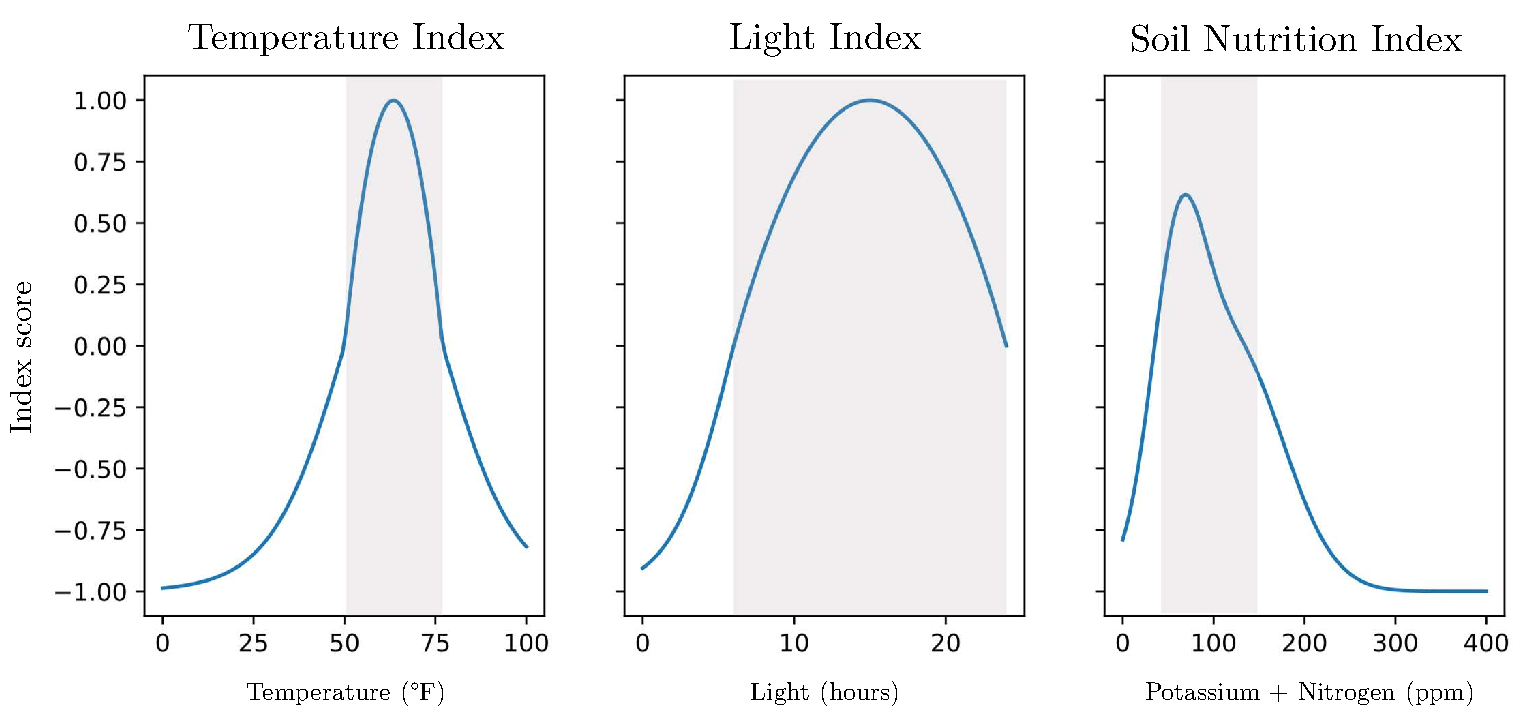
\includegraphics[scale=0.5]{figures/scoreindex.pdf}
    \captionsetup{width=0.9\textwidth}
    \caption{\textbf{From the left to right: \(T_I, L_I, N_I\) scores for plant growth.} Each shaded area represents the optimal interval for each unit of measure, which receives a positive score.}
    \label{fig:indexscoregraphs}
\end{figure}

\subsection{Seed Agent Model Overview}

Our method of modeling the spread of dandelions from an agent-based perspective is summarized in Figure~\ref{fig:partadiagram}.

\begin{figure}[htbp]
\centering
    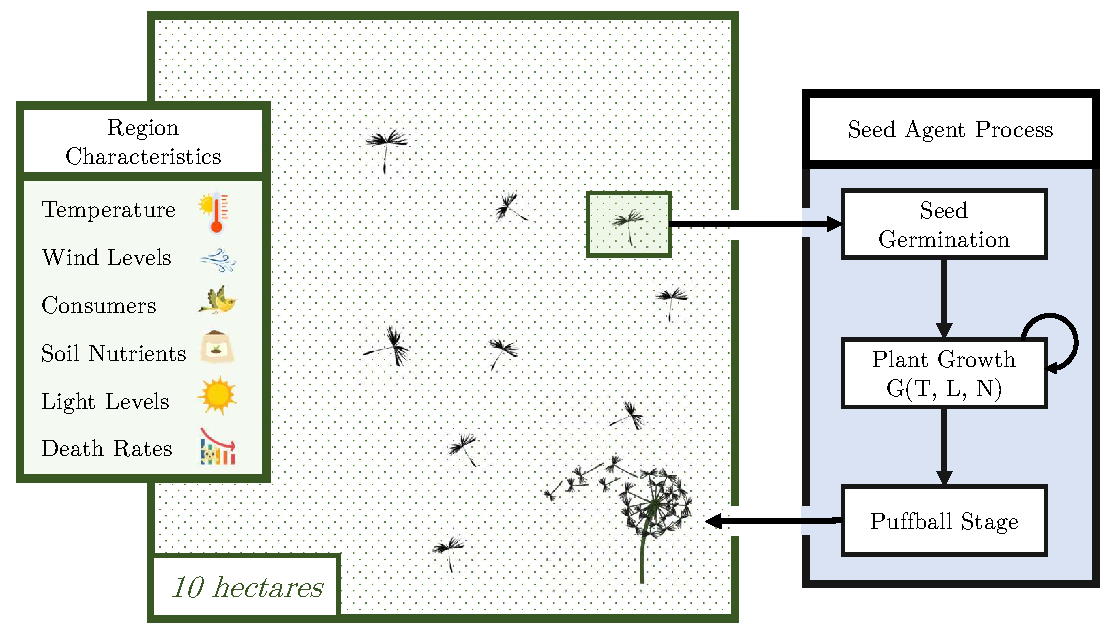
\includegraphics[scale=0.8]{figures/seedspreadprocess2.pdf}
    \captionsetup{width=0.9\textwidth}
    \caption{\textbf{Overview diagram of seed spread modeling.} }
    \label{fig:partadiagram}
\end{figure}

\section{Application of Agent-Based Model}

To simulate our agent-based model in real-world scenarios, we chose three distinct plots of land from a temperate, arid, and tropical region with relatively low human interference. So, we randomly selected three "open" regions in the United States. The regions selected for the temperate, arid, and tropical regions are Clay, New York; Phoenix, Arizona; and Florida Keys, Florida, respectively. 

\subsection{Climate Calibration}

To calibrate our model to each selected region, we define several of our \textit{hyperparameters} from the previous section, which capture the difference in climate, consumers, and soil nutrition levels. We use the term hyperparameters to designate global values that are not directly passed into our model but still change the output of the model. 

\begin{itemize}
    \item Temperature — The local temperature (\(^\circ\)F) over 2022.
    \item Light Levels — The local average hours of sunshine over 2022.
    \item Potassium and Nitrogen Levels — Local potassium and nitrogen levels (ppm) in the local soil. (Note that since Potassium levels are closely correlated with soil moisture, we did not choose to calibrate our model with rainfall, as potassium was indicative enough).    
\end{itemize}

See Appendix 1 for more details on the implementation of our agent-based simulation. 

\subsection{Regional Results}

\subsubsection{Temperate Region: Clay, NY}
We obtained data detailing the local temperature, light level, soil composition, and wind data of Clay, NY to calibrate our model's \textit{regional hyperparameters} \cite{aladin_wolcott_nodate, us_department_of_commerce_nowdata_nodate}. Our results for this region are summarized in Figure~\ref{fig:temperatespread} where \(t\) represents time and \(n\) represents the number of dandelions. Additionally, the graphs are scaled to the dimensions of the open plot of land we began with (100 meters by 100 meters). Recall that our first dandelion started at coordinate \((0,0)\).

\begin{figure}[h!]
\centering
    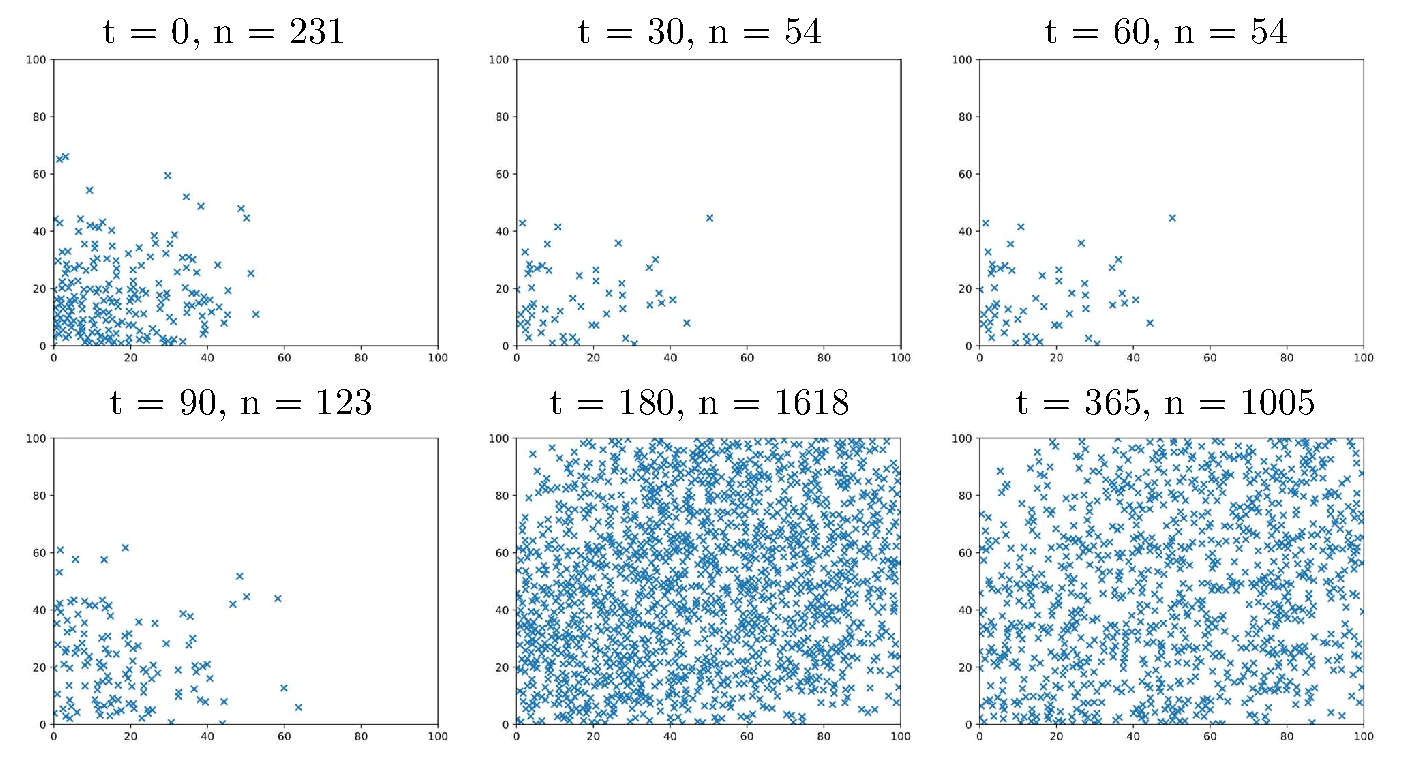
\includegraphics[scale=0.5]{figures/moderateclimatespread.pdf}
    \captionsetup{width=0.9\textwidth}
    \caption{\textbf{Dandelion spread over one year in Clay, NY.} Each mark labels a spot where a dandelion (either in seed or plant phase) is located at that time stamp \(t\).}
    \label{fig:temperatespread}
\end{figure}

One exciting observation is that the stochastic seed dispersal process seems to cover the plot of land over time uniformly. However, it is essential to note that \textit{not all seeds survive} the dispersal process. After 30, 60, and 90 days of simulation from the beginning of the calendar year, the seeds began to travel even farther from the starting point. At the 180-day mark, we see an influx of seeds and dandelion plants due to the effects of optimal climate conditions for a dandelion's blooming phase. After the blooming phase, we see that through day 365, all surviving agents that are left are plants in their dormancy stage.

\begin{figure}[h!]
\centering
    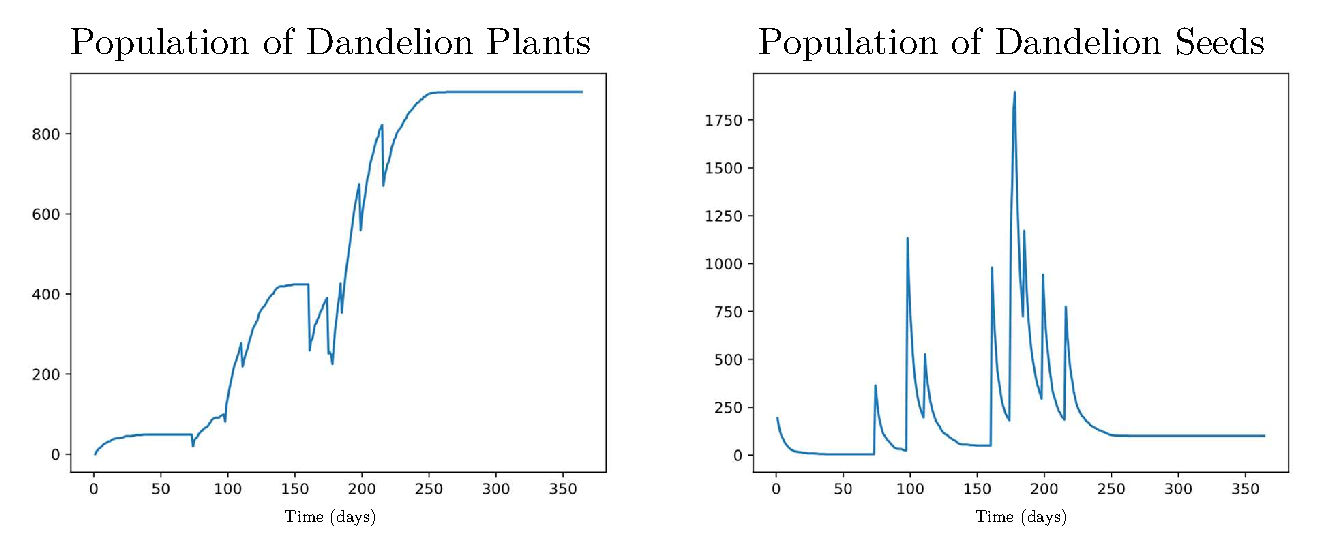
\includegraphics[scale=0.5]{figures/moderateclimatepopulation.pdf}
    \captionsetup{width=0.9\textwidth}
    \caption{\textbf{Growth in population of dandelion plants and seeds over time in Clay, NY.} The simulation began with a single puffball at coordinate \((0, 0)\).}
    \label{fig:temperatepopulation}
\end{figure}

A visualization of the growth (Figure~\ref{fig:temperatepopulation}) of the dandelion population and seed population over time shows us two key results:

\begin{enumerate}
    \item Dandelion plants go through two main blooming processes (spikes in population increase) throughout a year (spring and summer), which is consistent with other findings \cite{noauthor_dandelion_nodate-2}.
    \item Dandelion plant populations remain dormant in winter and fall months, while dandelion seeds do not spread much, or at all, in the colder months, which is a unique property of perennial plants \cite{noauthor_dandelion_nodate-2}.
\end{enumerate}

\subsubsection{Arid Region: Phoenix, AZ}

In Phoenix, Arizona, we obtained new climate and soil nutrition data from several sources \cite{arizona_guide_nodate, ottman_arizona_nodate, noauthor_average_nodate}. We then re-calibrated our model with these new hyperparameters and ran our simulated model.

\begin{figure}[h!]
\centering
    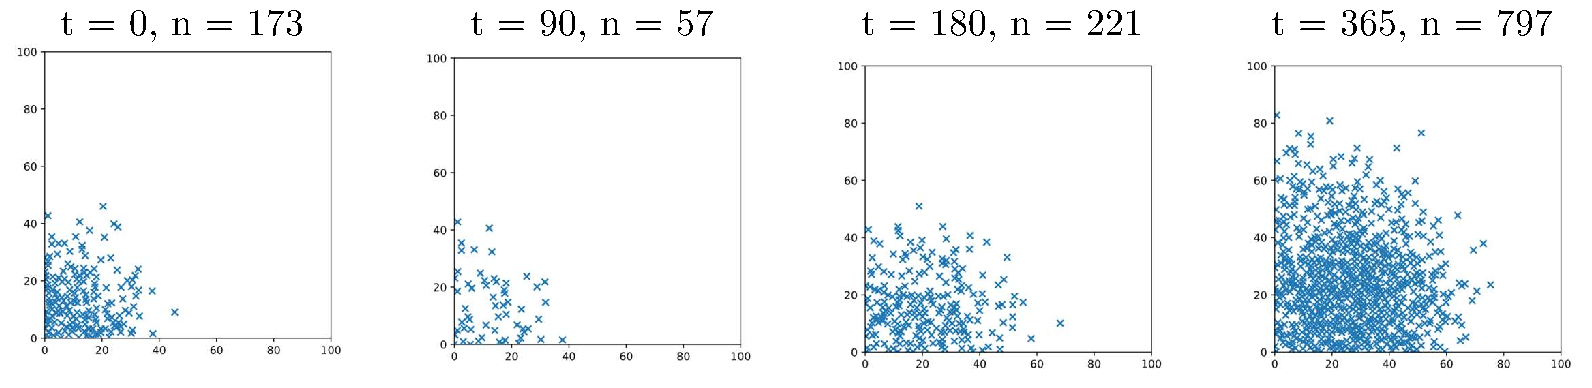
\includegraphics[scale=0.6]{figures/arizonaspread.pdf}
    \captionsetup{width=0.9\textwidth}
    \caption{\textbf{Dandelion spread over one year in Phoenix, Arizona.}}
    \label{fig:arizonaspread}
\end{figure}

\begin{figure}[h!]
\centering
    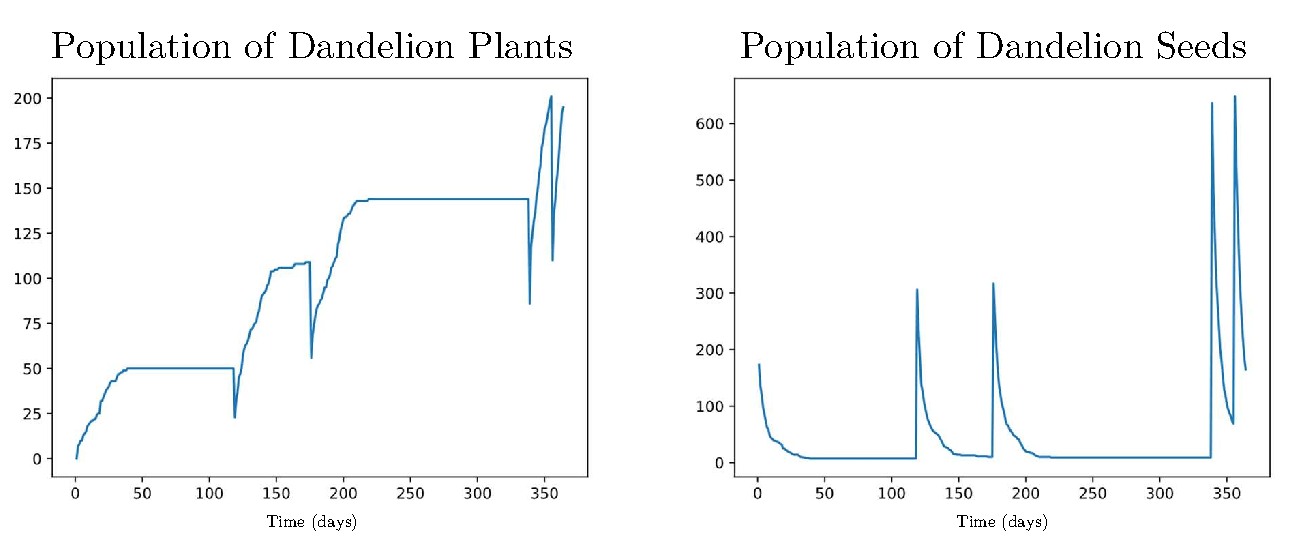
\includegraphics[scale=0.5]{figures/arizonapopulation.pdf}
    \captionsetup{width=0.9\textwidth}
    \caption{\textbf{Dandelion plant population growth in Phoenix, Arizona.}}
    \label{fig:arizonapopulation}
\end{figure}

One captivating observation of the spread of dandelions in an arid region is that their blooming seasons occur at different times of the year. This is most likely due to the availability of soil nutrients and optimal temperatures in the ending months of each year.

\subsubsection{Tropical Region: Florida Keys, FL}

By calibrating our model to Florida's tropical climate in the Florida Keys, we arrived at the following results for the dandelion growth and spread over one year. The calibrated climate data points were pulled from numerous sources as listed \cite{obreza_importance_2003, noauthor_average_nodate-1, pritchett_nitrogen_1959}.

One riveting observation of tropical regions is that blooming seasons tend to occur during winters at \(60-70^\circ\)F. Furthermore, we see that dandelion populations remain mostly stagnant over the summer months, as the summer heat may take away from dandelion growth. We can also conclude that dandelion populations follow a logistic growth pattern for the most part, which will be revisited in the following impact score model.

\begin{figure}[h!]
\centering
    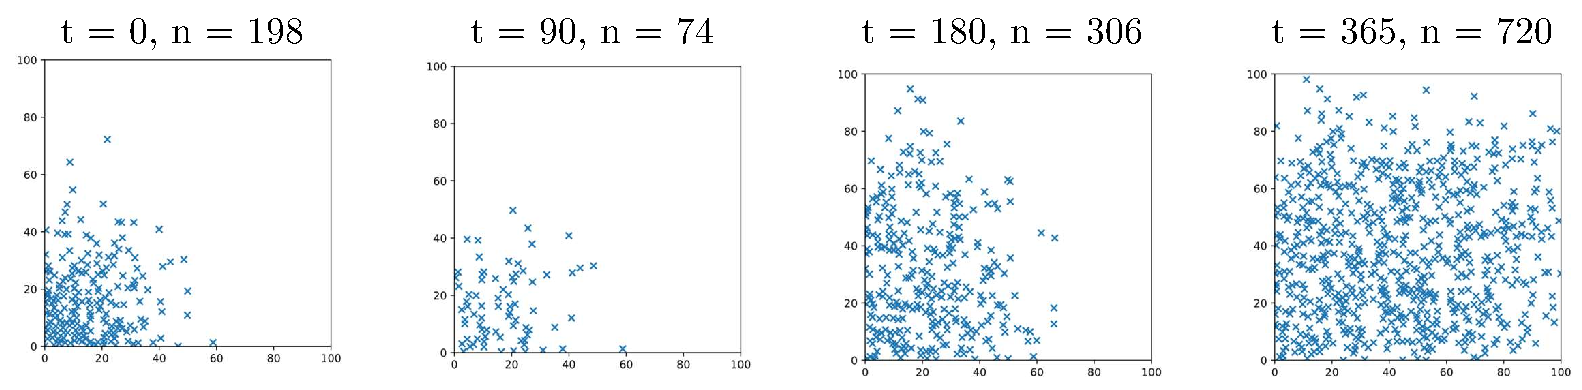
\includegraphics[scale=0.6]{figures/floridadistributions.pdf}
    \captionsetup{width=0.9\textwidth}
    \caption{\textbf{Dandelion spread over one year in Florida Keys, Florida.} }
    \label{fig:floridaspread}
\end{figure}

\begin{figure}[h!]
\centering
    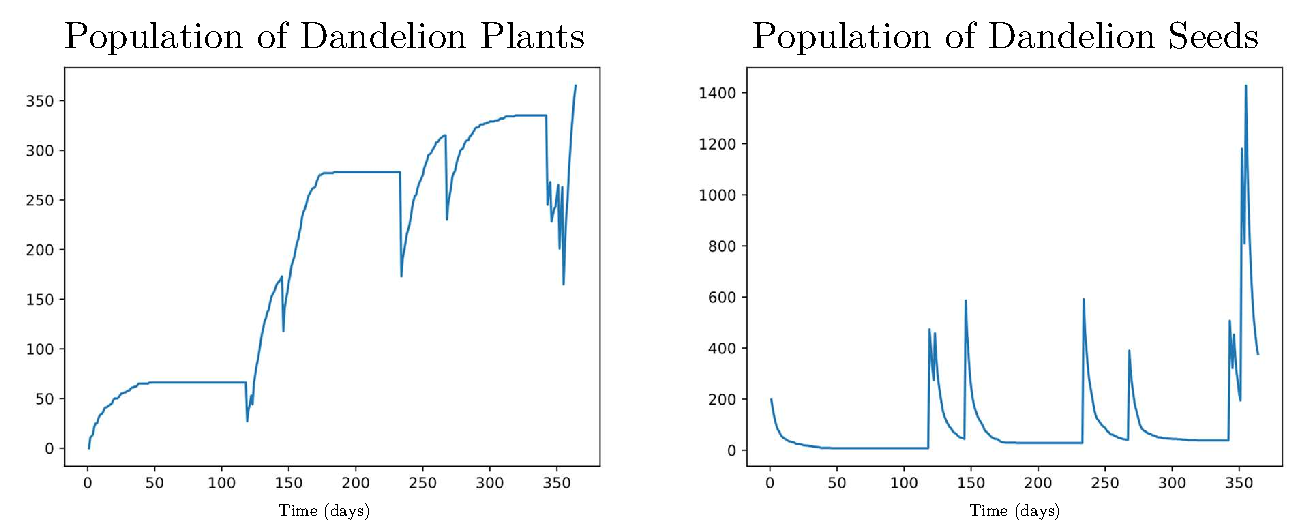
\includegraphics[scale=0.5]{figures/floridapopulation.pdf}
    \captionsetup{width=0.9\textwidth}
    \caption{\textbf{Dandelion plant population growth in Florida Keys, Florida.}}
    \label{fig:floridapopulation}
\end{figure}



\section{Model Discussion}

As a part of the creation of our agent-based model, where numerous climate and regional factors contribute to the spread of dandelion plants, we found it essential to conduct a sensitivity analysis to determine the most impactful factors on dandelion growth. Beyond our sensitivity analysis, we also provide a brief discussion of our model's key strengths and weaknesses, as well as a scope of how our model can be readily generalizable to virtually any plot of land.

\subsection{Model Hyperparameters}

The following table consolidates all hyperparameters based on our model described above. Our sensitivity analysis therefore investigates the impacts of these hyperparameters on the spread of dandelion plants and seeds.

\begin{table}[h!]
\renewcommand{\arraystretch}{1.3}
%p{0.8\linewidth
    \begin{tabularx}{\textwidth}{p{0.18\textwidth}lp{0.45\textwidth}X}
    \toprule
    \textbf{Hyperparameter}  & \textbf{Symbol} & \textbf{Description} & \textbf{Default Value} \\ \midrule
    \raggedright Temperature & \(\tau(t)\)   & Temperature (\(^\circ\)F) over a year in a specific region. Dandelions grow optimally between \(50-77^\circ\) F \cite{noauthor_dandelion_nodate-2}. & Temperatures of Clay, NY (2022) \cite{aladin_wolcott_nodate}. \\
    \rowcolor{gray!15}
    \raggedright Light Levels & \(l(t)\)  & Hours of sunlight per day over a year. Dandelions grow best between 6-24 light hours per day \cite{stewart-wade_biology_2002}. & Daily hours of light of Clay, NY (2022) data \cite{aladin_wolcott_nodate}.\\
    \raggedright Wind Levels & \(m(t)\) & Average mph of wind per day over a year which affects movement processes. & Wind levels in Clay, NY (2022) \cite{aladin_wolcott_nodate}. \\
   \rowcolor{gray!15} \raggedright K Levels & \(k(t)\) & Average amount of potassium in a regionally collected sample of soil in ppm over time. K levels account for soil moisture and richness \cite{noauthor_potassium_nodate}. & K levels from a soil survey \cite{communications_interpreting_2018}.\\
      \raggedright N Levels & \(n(t)\) & Average amount of Nitrogen (ppm) over time in a regionally collected sample of soil. & N levels from a soil survey \cite{pritchett_nitrogen_1959}.\\
    \rowcolor{gray!15} \raggedright Seed Lifespan & \(\lambda_s(t)\) & Average time until death for dandelion seeds. & 4 days \cite{noauthor_dandelion_nodate}. \\
    \raggedright Dandelion Lifespan & \(\lambda_d(t)\) & Average time until death for dandelion plants. & 15 days \cite{farmshowGrowingDandelions}. \\
     \rowcolor{gray!15} \raggedright Initial Seeds & \(S_0\) & Number of seeds dispersed by each puffball. & 2000 seeds \cite{noauthor_dandelion_nodate-2}. \\
    \bottomrule
    \end{tabularx}
\end{table}

\subsection{Sensitivity Analysis}

A standard methodology for sensitivity analysis is to randomly sample various values and analyze the model's output. Therefore, to randomly examine different sets of hyperparameters for our model, we employed a Monte Carlo sampling simulation to randomly sample \(\pm 10\%\) of default values. Based on the simulation, we modeled the effects of these changes on the growth of dandelion plant populations over time. These results are shown in Figure~\ref{fig:sensitivitypopulation}.

\begin{figure}[h!]
\centering
    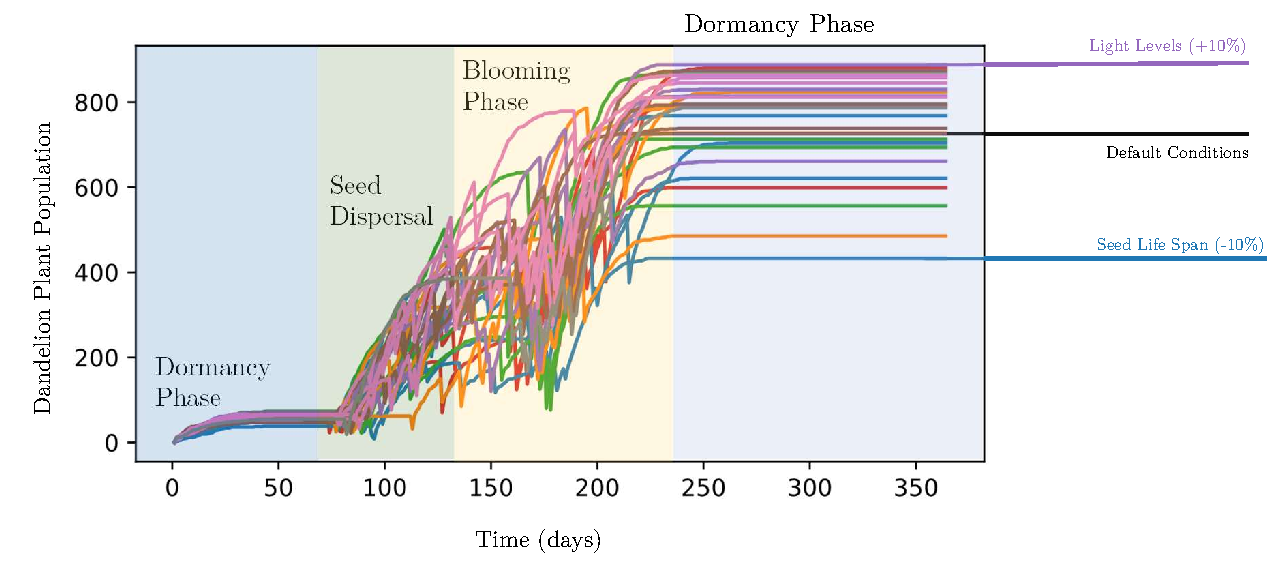
\includegraphics[scale=0.7]{figures/sensitivitypopulation.pdf}
    \captionsetup{width=0.9\textwidth}
    \caption{\textbf{Monte Carlo simulation sampling for hyperparameter sensitivity.}}
    \label{fig:sensitivitypopulation}
\end{figure}

In Figure~\ref{fig:sensitivitypopulation}, we demonstrate how, despite changes in our model's hyperparameters, dandelion populations tend to follow the same three-part process of dormancy, seed dispersal, and puffball blooming. At the end of the blooming phase, seeds are dispersed until the next blooming season reoccurs. Furthermore, dandelion plant populations generally approach an asymptote known as the carrying capacity of the plot of land, which in our case, is dependent on a hyperparameter specifying the minimum distance between two dandelions necessary to survive.

To numerically analyze our results from Figure \ref{fig:sensitivitypopulation}, we analyzed the average Root-mean squared error (RMSE) between each factor's Monte Carlo simulation and our simulation with default conditions applied. The RMSE formula is commonly used in time-series analysis to determine the average deviation of a new time series from a ground-truth series \cite{calzone_mae_2022}. 

\begin{equation}
    \text{RMSE} = \sqrt{\frac{1}{N}\sum\limits_{i=1}^{N} \left(x_{\text{new}_i} - x_{\text{ground truth}_i}\right)^2}
\end{equation}

Using the formula for RMSE where \(N\) is the number of entries compared, we scaled each of these errors between \(0\) and \(1\) using min-max scaling and displayed our sensitivity analysis results in the radar chart below. Based on our analysis, light levels and seed lifespan have the most significant impacts on dandelion population growth (See Figure~\ref{fig:radarchart1}), which is consistent with findings from field observations \cite{chepil_germination_1946}.

\begin{figure}[h!]
\centering
    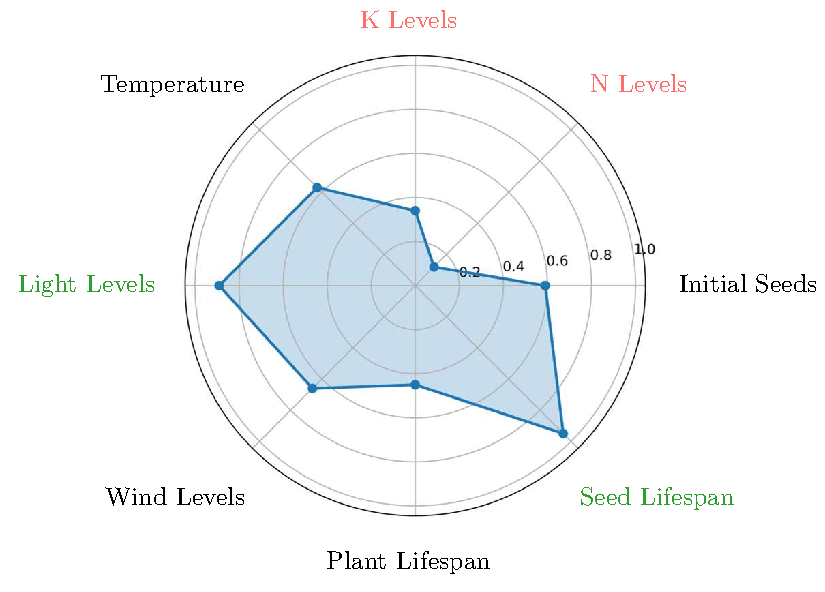
\includegraphics[scale=0.6]{figures/radarchart2.pdf}
    \captionsetup{width=0.9\textwidth}
    \caption{\textbf{Radar chart of model hyperparameters.} The two most impactful factors of our model were light levels and seed lifespan, but nutrient levels were least significant.} 
    \label{fig:radarchart1}
\end{figure}

\subsection{Strengths}

\begin{enumerate}
 \item Our model’s main strength is its ability to \textbf{powerfully generalize}.
    \begin{quote}
        For instance, by including numerous regional and climate hyperparameters into a single, robust framework, our model enables any investigator to thoroughly examine a plot of land for the growth of dandelions. Furthermore, all hyperparameters necessary can be easily obtained from open-access soil samples and climate analysis.
    \end{quote}
\item  Our model employs both \textbf{deterministic and probabilistic} techniques.
\begin{quote}
    Our model reflects real-life behavior of a cyclic dandelion population growth pattern and allows for stochastic variation in dandelion movement and growth.
\end{quote}

\item A thorough Monte Carlo simulation and sensitivity analysis performed \textbf{helps dandelion growers} and harvesting firms best grow dandelions through our analysis of impact factors.
\begin{quote}
    Our analysis concluded that light levels and seed lifespans impact dandelion growth the most; therefore, dandelion harvesters must prioritize these factors above all others to ensure that dandelions can grow most optimally.
\end{quote}
\end{enumerate}

\subsection{Limitations}
\begin{enumerate}
\item Some special data for dandelions could not be found, and so we assumed \textbf{that seeds act as independent agents} and follow growth cycles based on some key climate parameters. 
\begin{quote}
    More abundant data resources can guarantee more robust accommodation for diverse climates in our models. For example, occurrences of natural disasters, significant human interference, and specific consumer-based behaviors would result in a more adept model. 
\end{quote}

\item Our model \textbf{derives climate and death rates from historical data}.
\begin{quote}
    Therefore, our model lacks predictive power for factors such as global warming and competition with other species. Despite this limitation, using stochastic processes ensures that our model tends toward realism while also maintaining model elegance.
\end{quote}
\end{enumerate}



%% MODEL 2 %% 

\section{Part 2: Invasive Species Trade-Off Model}

[give more background on invasive species and their tradeoffs]
In the following section, we define \textit{foreign species} to be a non-native species that was just introduced to a new region of interest. Furthermore, we define \textit{spreadability} as the ease that a foreign species can spread on a new, rural plot of land.

\subsection{Problem Analysis}

Regarding the problem as a score calculation problem, a common first instinct to address this issue of developing an invasive species impact score is to divide the impact score into two primary categories: ecological impact and economic potential. With an all-encompassing model aimed to determining the impacts of a given species, we employ trade-off model between these two important criteria to support a classification of whether a foreign species truly is invasive. Figure~\ref{fig:invasiveimpactbrainstorm} illustrates an overview of our impact model.

\begin{figure}[h!]
\centering
    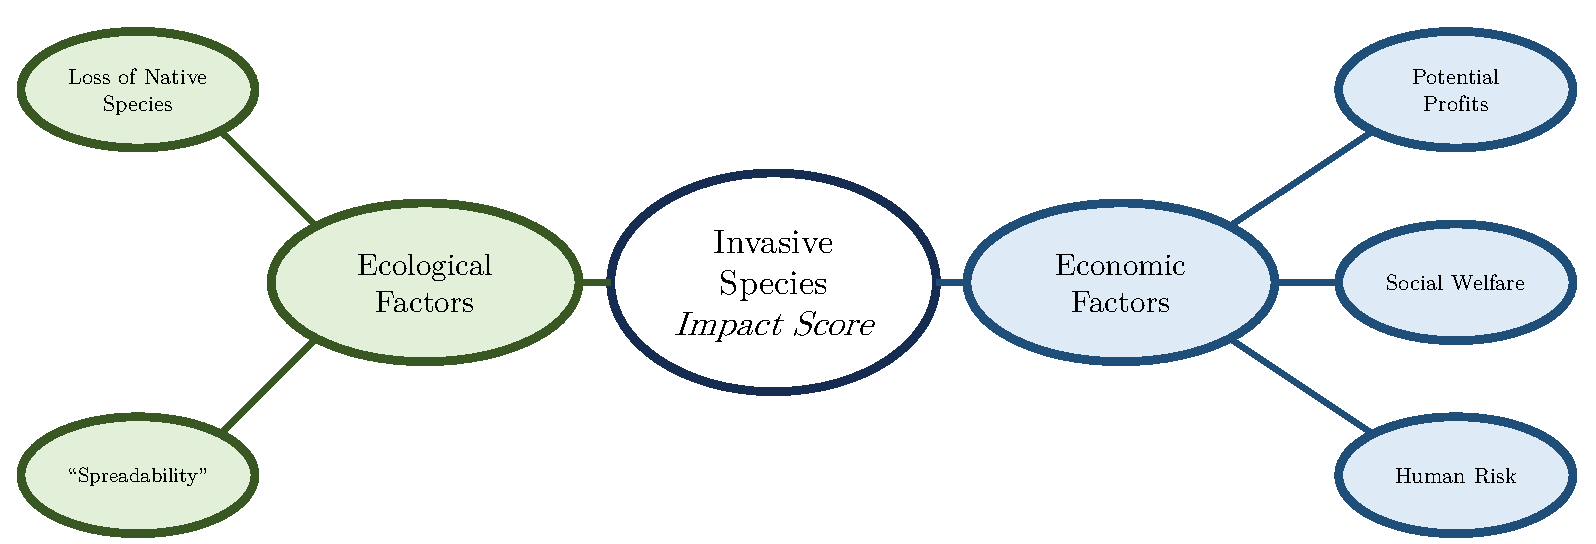
\includegraphics[scale=0.5]{figures/invasivespeciesimpactscore.pdf}
    \captionsetup{width=0.9\textwidth}
    \caption{\textbf{Overview of trade-off model.}.}
    \label{fig:invasiveimpactbrainstorm}
\end{figure}

\subsection {Assumptions}

Below, we list several core assumptions that allowed us to develop a trade-off model between ecological concerns and economic benefits. 

\begin{table}[h!]
\renewcommand{\arraystretch}{1.3}
    \begin{tabularx}{\textwidth}{lp{0.35\textwidth}X}
    \toprule
    \textbf{\#} & \textbf{Assumption} & {\centering \textbf{Justification}}  \\ \midrule
    
    \raggedright \nextassumption\label{assumption:10} & Native species prior to the introduction of a foreign species were in competitive equillibrium. & This key assumption allows us to use the Lotka-Volterra equations to compare before and after effects.\\
    
    \rowcolor{gray!15} \raggedright \nextassumption\label{assumption:11} & Foreign species follows a logistic growth with a set carrying capacity. & If a foreign species grows logistcally, we are able to create a standardized metric based on logistic regression for measuring population growth.
 \\

 \raggedright \nextassumption\label{assumption:12} & A foreign species social benefit and human health risk can be measured in dollars. & In being able to convert arbitrary ideas such as human health risk and social benefit to dollars, we are able to provide another standardized framework for these measures of impact. \\
 
    \bottomrule
    \end{tabularx}
\end{table}

\subsection{Variables}

The following list of variables summarizes the key components of our trade-off model. We will derive each of the following functions (or scores) in this section.

\begin{table}[h!]
\renewcommand{\arraystretch}{1.3}
%p{0.8\linewidth
    \begin{tabularx}{\textwidth}{p{0.25\textwidth}lX}
    \toprule
    \textbf{Variable}           & \textbf{Symbol} & \textbf{Description}  \\ \midrule
    \raggedright Native Species Population Changes & $\chi$  & Sum of proportions of changes in native species populations before and after introduction of foreign species. \\
    \rowcolor{gray!15}
    \raggedright Spreadability Rate  & $r$  & Rate of growth of foreign species by itself based on logistic regression. \\
    Economic Profit & $\pi$  & Potential profit (in dollars) made in a business centered around an foreign species. \\
    \rowcolor{gray!15} \raggedright Social Welfare Benefit& $W$   &  External social benefit not from direct harvesting of an foreign species. \\
    \raggedright Human Health Risk & $R$ & Potential risk in dollar-value cost of an foreign species to humans.\\
    \bottomrule
    \end{tabularx}
\end{table}

\subsection{Ecological Impact Score}

As a first step, we broke down our first part of the score, the ecological impact score, into three distinct categories. Regarding species to be classified as invasive, several factors are essential to consider, such as detrimental impact to native plants, the species' ability to spread (spreadability), risk to human health, and risk to native soil nutrition. Therefore, we propose an ecological impact score as a combination of these factors, none of which are dispositive. 

\subsubsection{Effects on Native Species}

To analyze the impacts of a non-native species in a new region, we need to measure the unintendend consequences in native populations. To do so, we take we used the Lotka-Volterra model (a system of differential equations) to represent the changes in population for each native species. The Volterra-Lotka model is commonly used for analyzing the population dynamics of competing species, especially in our case between nonnative and native species. 

Assuming native species are in competitive equillibrium prior to the introduction of a new non-native species (Assumption~\ref{assumption:10}), we can use a generalized set of Lotka-Volterra equations for \(n\) native species, where we can treat population growth for each species as a single vector based on the populations of other species at each time step. Furthermore, the weightings of how other native species populations affect the growth of another species can be stored in a matrix.

In mathematical terms, let there be \(n\) native species where population of a native species \(i\) where \(1 \leq i \leq n\) is denoted by \(x_i\). Therefore, the rate of change of a population \textit{in relation to} other species can be represented as 

\begin{equation}
    \frac{dx_i}{dt} = r_ix_i \left(1 - \frac{\sum\limits_{j=1}^n \alpha_{ij} x_j}{K_i}\right)
    \label{eq:lotkavolterra}
\end{equation}

where \(r_i\) is the internal growth rate of species \(i\), \(\alpha_{ij}\) is the impact of species \(j\) on species \(i\), and \(K_i\) is the carrying capacity of species \(i\). The parameters \(\alpha_{ij}\) can be combined into an \(i\) by \(i\) matrix of "interaction" parameters, therefore we denote this matrix of parameters the \textit{interaction matrix}. For the first \(n\) native species, the Lotka-Volterra equation will yield a system of \(n\) differential equations with an \(n\) by \(n\) matrix \(\alpha\). When we introduce our new foreign species, the Lotka-Volterra model will yield a system of \(n+1\) differential equations with an interaction matrix \(\alpha\) of dimensions \(n+1\) by \(n+1\) where all values \(\alpha_{ii} = 1\) for self-interaction of species.

Based on the data readily available for our use, we determined that understanding the changes in populations of 3 native species for each foreign species would be sufficient. To create a standardized score, however, we propose a native population impact score which measures \textit{ratio} of a native species prior to and after 1 year (365 days) since the introduction of a new foreign species. Therefore, let our native species impact score \(\chi\) be the sum of the ratios of native population species before and after the introduction of foreign species. Therefore, we can define our native species impact score \(\chi\) as 

\begin{equation}
    \chi = \sum_{i = 1}^n \frac{x_i {\text{ new}}}{x_i {\text{ old}}}
    \label{eq:nativepopratio}
\end{equation}

With the use of scientific software such as SciPy \cite{scipy}, we can obtain a numerical solution to this system to analyze the changes in native species population over time.

\subsubsection{Spreadability Index}

To measure spreadability, we focus on the ability of a population to regenerate and grow without competitors and with optimal access to natural resources. Regarding population growth as an logistical growth problem (See Assumptionn~\ref{assumption:11}), we develop a standardized logistic regression model to evaluate the \textit{spreadability} of a species. As most populations follow a logistic growth pattern with an ultimate environmental carrying capacity, we are able to generalize this process to most, if not all common species.

Based on historical population growth data throughout a year in an optimal setting, we can perform logistic regression on population data, such that the population data of a species can be best modeled by a function 

\begin{equation}
    N(t) = \frac{L}{1+Ce^{-rt}}
\end{equation}

for carrying capacity \(L\), constant \(C\), and proportionality constant of growth \(r\). Since \(r\) can easily describe the proportion of growth over a continuous time interval, we let our \textit{spreadability index} be the value \(r\) properly scaled by a factor of 100. So, our spreadability index can be represented as \(100r\). Therefore, we can represent the ecological impact score the sum of \(\chi\) from \(100r\) as the greater the loss in native species, the greater the ecological impact score gets.  Note that the we are looking for a lower ecological impact score of a species.

\begin{equation}
    \text{Ecological Impact Score } = 100r + \chi
    \label{eq:ecologicalimpact}
\end{equation}


\subsection{Potential Economic Potential}

Based on Assumption~\ref{assumption:12}, we primarily considered a standardized measure for analyzing the economic benefits and downfalls: monetary value. 

\subsubsection{Net Profit}

In the context of bioeconomics, a common model used to analyze the production value and potential maximum yield and profit from harvesting a specific species is called the Gordon-Schaefer Model \cite{wikipediaGordonSchaeferModel}. Gordon-Schaefer bioeconomic analysis methods can be applied whenever a species follows a logistic growth pattern, where a population levels off to some carrying capacity based on its respective environment. From the first model analyzing dandelion spread, we can see that indeed dandelions satisfy this key assumption, therefore we can apply the Gordon-Shaefer model respectively.

To find the maximum sustainable profit of an industry centered around harvesting a specific species, we can apply the microeconomic \textit{Profit Maximization Law}, where the optimal level of harvest, otherwise known as the maximum sustainable yield, can be found at the intersection of \textit{marginal revenue} and \textit{marginal cost} (MR=MC) \cite{intelligenteconomistProfitMaximization}.

In the context of a Gordon-Schaefer harvesting model, marginal revenue can be interpreted as the revenue per unit of effort in harvesting, and marginal cost can be interpreted as the cost to harvest each unit of species. As the marginal revenue decreases over time due to the Law of Diminishing Marginal Returns \cite{investopediaDiminishingMarginal}, we will calculate the optimal yield effort at the intersection of the MR and MC curve, then find that corresponding point on a \textit{Total Revenue} and \textit{Total Cost} curve to obtain the maximum profit (\(\pi\)). See Figure~\ref{fig:gordonschafer} for a visual representation of the process. Note that each species will have a Gordon Schaefer bioeconomic model calibrated to it based on industry data.

\begin{figure}[h!]
\centering
    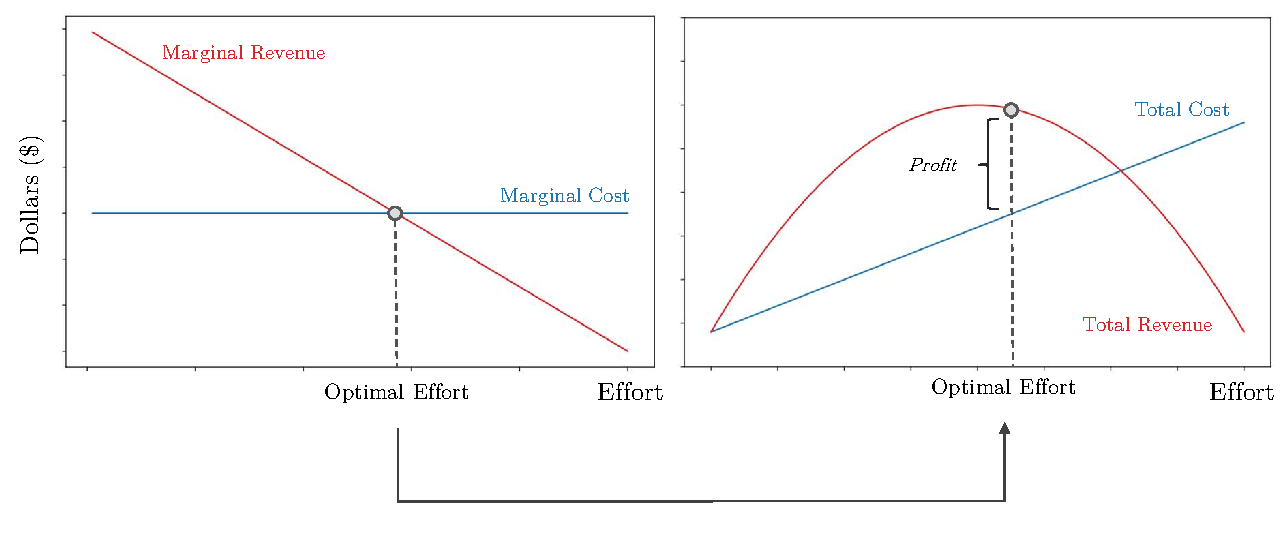
\includegraphics[scale=0.65]{figures/gordonschaefer.pdf}
    \captionsetup{width=0.9\textwidth}
    \caption{\textbf{Gordon-Schaefer model effort optimization for species harvesting.} Note that Net Profit (\(\pi\)) for the harvesting of a species can be obtained from the difference between Total Revenue and Total Cost.}
    \label{fig:gordonschafer}
\end{figure}

\subsubsection{Social Benefit}

To calculate social welfare benefit of a foreign species on society, or in more economic terms, positive externalities, we can calculate the \textit{total social welfare} received by a population surrounding the foreign species and region in question. In order to determine the explicit dollar-value benefits of social welfare, we can utilize Sen's Welfare Function (which incorporates a Gini coefficient) to model the benefits of a certain species scaled to the region's income inequalities \cite{wikipediaSocialWelfare, worldbankWorldBank}. 

Therefore, we can express the \textit{total welfare benefit} (in dollars) \(W\) as a sum of individual benefits \(Y_i\), Gini coefficient \(G\), and regional population \(n\),

\begin{equation}
    W = (1 - G) \sum_{i=1}^n Y_i
\end{equation}

\subsubsection{Human Health Risk}

To calculate human health risk as an economic factor, we analyze the average detriment a species has to humans as a sum of individual risks based on the potential amount of money lost. The sum can again be scaled similar to Sen's Welfare Function using the Gini coefficient. Data for the detrimental costs of a species to human society can be found for virtually any species, therefore, allowing us to make the assumption for generalizability.

Therefore, we express the \textit{total human risk} (in dollars) \(R\) as a sum of individual risks \(R_i\), Gini coefficient \(G\), and regional population \(n\),

\begin{equation}
    R = (1 - G) \sum_{i=1}^n R_i 
\end{equation}

Therefore, we can express the total economic benefit of a given species in a region to be the sum of economic profit and social benefit minus the human health risk.

\begin{equation}
    \text{Total Economic Benefit } = \pi + W - R
    \label{eq:economicimpact}
\end{equation}

where \(\pi\) is the maximum profit yield, \(W\) is the social welfare benefit, and \(R\) is the total human health risk. 

So, our combined foreign species trade-off score can be determined as a coordinate pair of two sub-scores: one ecological (Equation~\ref{eq:ecologicalimpact}), one economic (Equation~\ref{eq:economicimpact}), which is shown as follows.

\begin{equation}
    \text{\textbf{Impact Score} } = (\text{Ecological Score, Economic Score}) = (100r + \chi, \hspace{0.05cm} \pi + W - R)
\end{equation}

\section{Application of Trade-Off Model}

By calculating our two scores, ecological and economic, we can apply our impact score calculations to virtually any invasive species. For the purposes of our discussion, our choice of three commonly-regarded-to-as invasive or foreign plants species from the United States region includes: \textit{dandelions} in New York, \textit{garlic mustard plants} in Illinois, and  \textit{English ivy} plants in Washington \cite{columbiatribuneDandelionsFight, natureGarlicMustard, invasiveEnglishHedera}.

[background on dandelion, garlic mustard, and English ivy plants]

\subsection{Dandelion Plants}
\subsubsection{Ecological Impact Score}

To first determine the ecological impact score of dandelion plants, we examine the top 3 closely-related native species where dandelions reside in New York, which include the following species.

\begin{itemize}
    \item \textbf{Bombus impatiens} (Bumblebees) — native pollinators common to eastern North America that commonly visit dandelion species to obtain pollen and help dandelions reproduce, therefore, they have a mutualistic relationship \cite{nwfCommonEastern}.
    \item \textbf{Malacosoma americanum} (Moths) — feeds on the leaves of the common dandelion in New York. A consumer-plant relationship with dandelions \cite{butterfliesandmothsEasternTent}.
    \item \textbf{Cuscuta gronovii} (Scaldweed) — a climbing parasitic vine that extracts nutrients from attached-to plants \cite{minnesotawildflowersCuscutaGronovii}.
\end{itemize}

Below, we determined an interaction matrix for the Lotka-Volterra model based on the interactions of each species in row \(i\) to the species in column \(j\). Therefore, each \(\alpha_{ij}\) represents the interaction of species \(j\) on species \(i\). For example, if species \(j\) was a natural predator of species \(i\), the value of \(\alpha_{ij}\) will be a negative value. If two species were mutualistic, we would expect that the element \(\alpha_{ij}\) would be indeed positive, thus improving the rate of growth of either population. Note that generally, element \(\alpha_{ij} \neq \alpha_{ji}\) because the effect species \(i\) has on species \(j\) is generally opposite to the effect in the reverse order. Furthermore, the impact of the invasive species on native populations is found in the fourth row and column of matrix \(\alpha\).

Assuming a starting population each of 100 plant units and a carrying capacity of 1000 plant units each, and growth rate of 0.005 for bumblebees, as their populations mostly fluctuate by seasons, 0.06 for moths as their populations grow quickly, 0.01 for vines as their populations tend to stabilize, and 0.04 for dandelions as show in the following logistic regression section \cite{nwfCommonEastern, butterfliesandmothsEasternTent, minnesotawildflowersCuscutaGronovii}. We solve the systems of differential equations show in Equation~\ref{eq:lotkavolterra} with the following interaction matrix approximated based on the relationships between each species.

\begin{equation}
        \alpha_{\text{ dandelion}} = {\underbrace{\begin{bNiceMatrix}[first-row,first-col]
        &&&&& \\
    \text{Bumblebees} && 1 & 0.25 & -0.5 & 2 &\\
    \text{Moths} && 0.25 & 1 & 0.6 & 0 &\\
    \text{Vines} && -0.5 & -0.5 & 1 & 2 &\\
    \text{Dandelions} && 2 & 0.25 & -1 & 1 & \\
    \end{bNiceMatrix}}_{ \\ \text{3 native species, 1 invasive species}}}
\end{equation}

From graphing the population solutions to the system, we can see the population shifts in Figure~\ref{fig:lotkavolterradandelion}. Based on the numerical solution to this differential equation from scientific computing software, we find the change of populations over a single year (365 days) to be \(\frac{1200}{100}\) for moths, \(\frac{250}{850}\) for vines, and \(\frac{550}{100}\) for bumblebees. So, we can calculate the native species impact score to be

\[\chi = \frac{1200}{100} + \frac{250}{850} + \frac{550}{100} = 17.794\]
%% need to do some graphing and calculations

\begin{figure}[h!]
\centering
    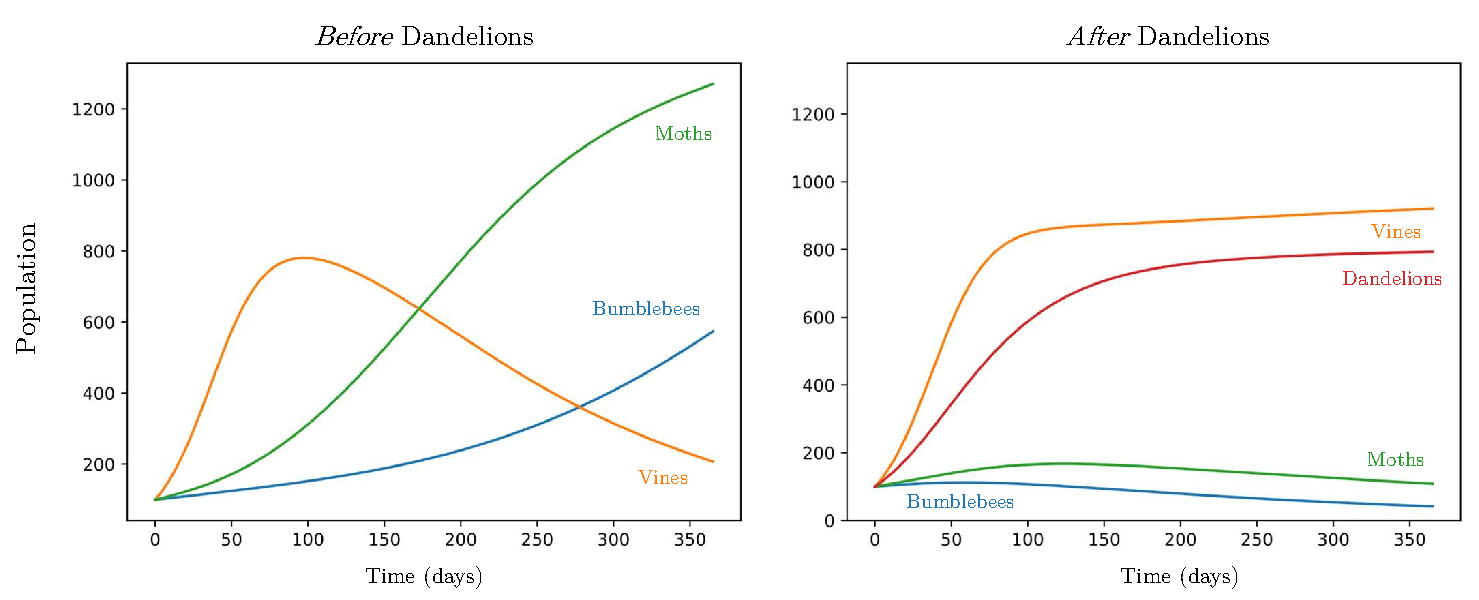
\includegraphics[scale=0.5]{figures/lotkavolterradandelions.pdf}
    \captionsetup{width=0.9\textwidth}
    \caption{\textbf{Before and after plot of native species populations of introduction of dandelion species}. Based on Lotka-Volterra competitor system of differential equations.}
    \label{fig:lotkavolterradandelion}
\end{figure}

Next, we calculate the spreadability index by performing logistic regression on dandelion data from the previous model. From plant population predictions in New York, we find that the carrying capacity of a region is approximately 900 dandelion plants, with a relatively logistic-shaped curve. Therefore, we calculate from logistic regression and finding the best-fit logistic curve, that the spreadability score (or proportionality of growth) is \(r = 0.04\), therefore our spreadability score is \(100r = 4\).

By Equation~\ref{eq:ecologicalimpact}, we see that our total ecological impact score is \(4 + \chi = 4 + 17.794 = 21.794\).

\subsubsection{Economic Potential}

To estimate economic profits, we assume there exists some small dandelion harvesting firm in New York. So, we proceed with analyzing the microeconomics of the business.

According to a variety of sources, we can approximate the marginal cost of harvesting each dandelion to be around \(\$0.10\) per unit of effort (to harvest one pound of dandelions) \cite{farmshowGrowingDandelions, gardeningknowhowDandelionHarvest}. We can approximate the marginal revenue curve by utilizing the fact that marginal revenue decreases for every five pounds of dandelions sold with maximum marginal revenue at around \(\$4.50\) per pound of dandelions \cite{farmfitlivingMakeMoney}. So, we can model marginal revenue with a linear model with slope -0.2 and y-intercept 4.5. From integration, we can calculate the the total revenue and total cost curve based on effort levels, which is shown in Figure~\ref{fig:dandelionprofits}. Therefore, we calculate dandelion profits (\(\pi_{\text{dandelions}}\)) be around \(\$47.86\).

\begin{figure}[h!]
\centering
    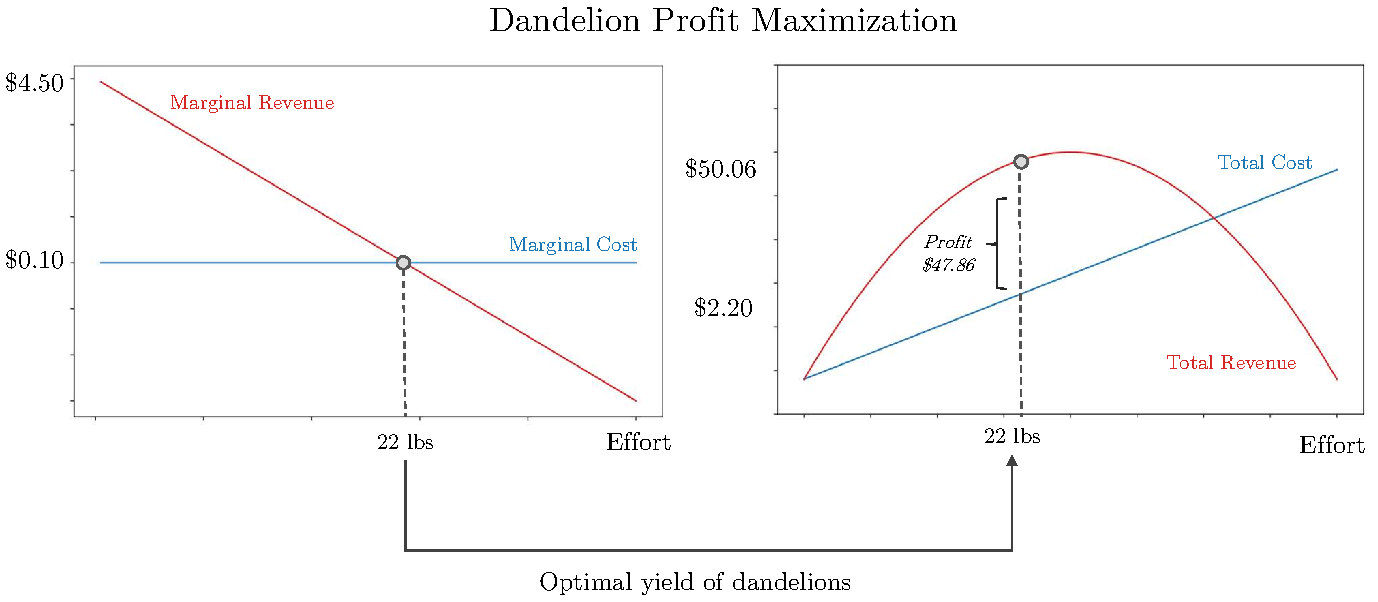
\includegraphics[scale=0.5]{figures/dandelionprofitmax.pdf}
    \captionsetup{width=0.9\textwidth}
    \caption{\textbf{Gordon-Schaefer model for dandelion profit yield.}}
    \label{fig:dandelionprofits}
\end{figure}

On top of calculating potential economic profits of a small dandelion business in New York, we additionally need to calculate the social welfare benefits and potential human risks. The average population of a New York town , is approximately \(n = 60,000\), and the net external benefit for each individual is approximately \(\$0.002\) as a rarely used medicinal plant and common soil loosener which can improve the growth of other harvested plants \cite{healthlineDandelionHealth}. Furthermore, for the New York, the Gini coefficient is 0.52 \cite{statistaBetweenRich}. Therefore, the social welfare output is \[W = (1- 0.52) \sum_{i = 1}^{60000} 0.002 = \$57.60\].

As a final part of calculating potential economic profits, we find the human health risk by calculating the amount of harm of a dandelion has on its surrounding human population. Since the only potential harm a dandelion could impose would be to people with dandelion allergies, we deduce that the potential human risk would be \(R = 0\).

With the three components of the economic potential score, we can calculate the score to be 

\[\text{Total Economic Benefit } = \pi + W - R = 47.86 + 57.60 - 0 = \$105.46\]

So, our final invasive species impact score is

\[\text{Impact Score} = (\text{Ecological Score, Economic Score}) = (21.794, \$105.46)\]

\subsection{Garlic Mustard Plants}

\subsubsection{Ecological Impact Score}

Next, to determine the ecological impact score of garlic mustard plants, we examine the top 3 closely-related native species where garlic mustard plants reside in Illinois, which include the following species.

\begin{itemize}
    \item \textbf{White trillium} (Wildflower) — native wildflower that grow in woodlands often threatened by garlic mustard invasion \cite{usdaGreatWhite}.
    \item \textbf{Plethodon cinerus} (Salamander) — amphibian that lives under leaves and forests and feeds on insects and other small inveterbrates \cite{amphibiawebAmphibiaWebPlethodon}.
    \item \textbf{Hylocichla mustelina} (Wood thush) — a songbird that nests in forests where garlic mustard invasion reduces vegetation for nesting cover \cite{allaboutbirdsWoodThrush}.
\end{itemize}

% https://extension.illinois.edu/invasives/garlic-mustard

Below, we again determined an interaction matrix for the Lotka-Volterra model based on the interactions of each species in row \(i\) to the species in column \(j\). Note that we again assume that the starting population of each species is units with a carrying capacity of 1000 plant units each, and a growth rate of 0.06 for wildflowers, as their populations mostly fluctuate by seasons, 0.03 for salamanders as their populations do not grow as quickly, 0.01 for songbirds as their populations tend to stabilize, and 0.1 for garlic mustard plants as their populations tend to grow very quickly. We solve the systems of differential equations show in Equation~\ref{eq:lotkavolterra} with the following interaction matrix approximated based on the relationships between each species.

\begin{equation}
        \alpha_{\text{ garlic mustard}} = {\underbrace{\begin{bNiceMatrix}[first-row,first-col]
        &&&&& \\
    \text{Wildflower} && 1 & 0.75 & 1.5 & -1 &\\
    \text{Salamanders} && 0.35 & 1 & 0.65 & -1 &\\
    \text{Songbirds} && 0.5 & 0.5 & 1 & -1 &\\
    \text{Garlic mustard} && 0.25 & 0.25 & 0.15 & 1 &\\
    \end{bNiceMatrix}}_{ \\ \text{3 native species, 1 invasive species}}}
\end{equation}

In the fourth column, since garlic mustard plants have a negative impact on all three of the native species populations, we assigned a value of -1 to each element. 

From graphing the population solutions to the system, we can see the population shifts in Figure~\ref{fig:lotkavolterragarlicmustard}. Based on the numerical solution to this differential equation from scientific computing software, we find the change of populations over a single year (365 days) to be \(\frac{100}{100}\) for wildflowers, \(\frac{800}{400}\) for salamanders, and \(\frac{400}{200}\) for songbirds. So, we can calculate the native species impact score to be

\[\chi = \frac{150}{100} + \frac{800}{450} + \frac{400}{200} = 5.278\]
%% need to do some graphing and calculations

\begin{figure}[h!]
\centering
    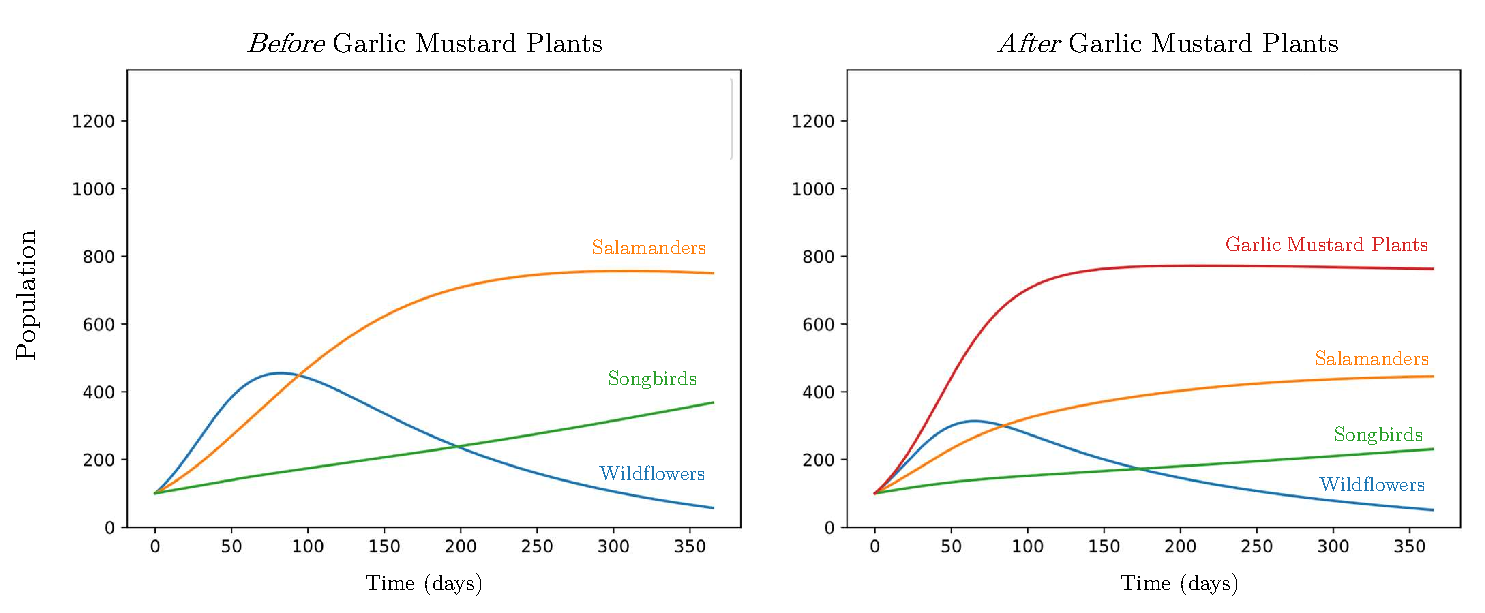
\includegraphics[scale=0.5]{figures/lotkavolterragarlicmustard.pdf}
    \captionsetup{width=0.9\textwidth}
    \caption{\textbf{Before and after plot of native species populations of introduction of Garlic mustard species}. Based on Lotka-Volterra competitor system of differential equations.}
    \label{fig:lotkavolterragarlicmustard}
\end{figure}

To calculate the spreadability index, we can start from a commonly regarded fact that Garlic mustard populations can double in a year in most growing conditions \cite{fmrInvasiveSpecies}. Therefore, by performing logistic regression with the x-axis being days and the y-axis as population, we can find that the \(r\) value is around 0.05. So, our spreadability index can be calculated as \(100r = 5\). Therefore, by Equation~\ref{eq:ecologicalimpact}, our ecological impact score is \(5 + \chi = 5 + 5.278 = 10.278\).

\subsubsection{Economic Potential}

As harvesting efforts for garlic mustard plants are minimal-to-none, we conclude that there is no possibility of a garlic mustard harvesting farm. This means that there is \textit{no potential economic profit} in a plot of land for a garlic mustard growth. Therefore, our economic profit \(\pi = 0\).

We additionally need to calculate the social welfare benefits and potential human risks of Garlic mustard plants. The population of an average town in Illinois, is approximately \(n = 50,000\), and the net external benefit for each individual is similar to dandelions at approximately \(\$0.002\) as a rarely used medicinal plant and herb \cite{fmrInvasiveSpecies}. Furthermore, for the Illinois, the Gini coefficient is 0.48 \cite{247wallstIncomeInequality}. Therefore, the social welfare output is \[W = (1- 0.48) \sum_{i = 1}^{50000} 0.001 = \$26.00\].

As a final part of calculating potential economic profits, we find the human health risk by calculating the amount of harm of population of garlic mustard plants has on its surrounding human population. Since garlic mustard plants are edible, the only potential harm a dandelion could impose would be to people with garlic mustard plant allergies, so we deduce that the potential human risk would be \(R = 0\) \cite{fmrInvasiveSpecies}.

With the three components of the economic potential score, we can calculate the score to be 

\[\text{Total Economic Benefit } = \pi + W - R = 0 + 26.00 - 0 = \$26.00\]

So, our final invasive species impact score for Garlic Mustard plants is

\[\text{Impact Score} = (\text{Ecological Score, Economic Score}) = (5.278, \$26.00)\]

\subsection{English Ivy Plants}

\subsubsection{Ecological Impact Score}
To deduce the ecological impact score of English ivy plants, we examine the top 3 most closely-related native species where English ivy plants reside in Washington, which include the following species.

\begin{itemize}
    \item \textbf{Kinnikinnick} (Shrub) — an evergreen shrub that grows in most conditions and attracts a variety of native pollinators and birds \cite{wnpsPlantProfile}.
    \item \textbf{Asarum caudatum} (Wild ginger) — a low lying groundcover plant with leaves and is edible for most herbivores \cite{portlandnurseryAsarumCaudatum}.
    \item \textbf{Mahonia aquifolium} (Oregon grape) — another evergreen plant that produces berries and can grow in most temperate conditions in Washington \cite{oregonstateMahoniaAquifolium}.
\end{itemize}

% https://www.gardeningknowhow.com/ornamental/groundcover/english-ivy/english-ivy-alternatives.htm

% https://www.nwcb.wa.gov/weeds/english-ivy

For the last time, we determined an interaction matrix for the Lotka-Volterra model. Note that we again assume that the starting population of each species is units with a carrying capacity of 1000 plant units each, and a growth rate of 0.02 for shrubs, as their populations mostly fluctuate by season, 0.04 for wild gingers as their populations grow rapidly across forest floors, 0.01 for Oregon grapes as their populations tend to stabilize, and 0.4 for English ivy plants as their populations tend to grow very quickly. We solve the systems of differential equations show in Equation~\ref{eq:lotkavolterra} with the following interaction matrix approximated based on the relationships between each species.

\begin{equation}
        \alpha_{\text{ English ivy}} = {\underbrace{\begin{bNiceMatrix}[first-row,first-col]
        &&&&& \\
    \text{Shrubs} && 1 & 0 & -0.5 & -0.25 &\\
    \text{Wild ginger} && 0 & 1 & 0 & -1 &\\
    \text{Oregon grape} && -0.5 & 0 & 1 & -1 &\\
    \text{English ivy} && 0.25 & -0.5 & 0.15 & 1 &\\
    \end{bNiceMatrix}}_{ \\ \text{3 native species, 1 invasive species}}}
\end{equation}

In several spots throughout the interaction matrix, the elements are set to zero because of the different habitats the plants occupy. That means, they rarely compete for the same nutrients in their local regions. However, English ivy plants compete strongly with wild ginger, as they both can grow along forest floors \cite{portlandnurseryAsarumCaudatum}.

\begin{figure}[h!]
\centering
    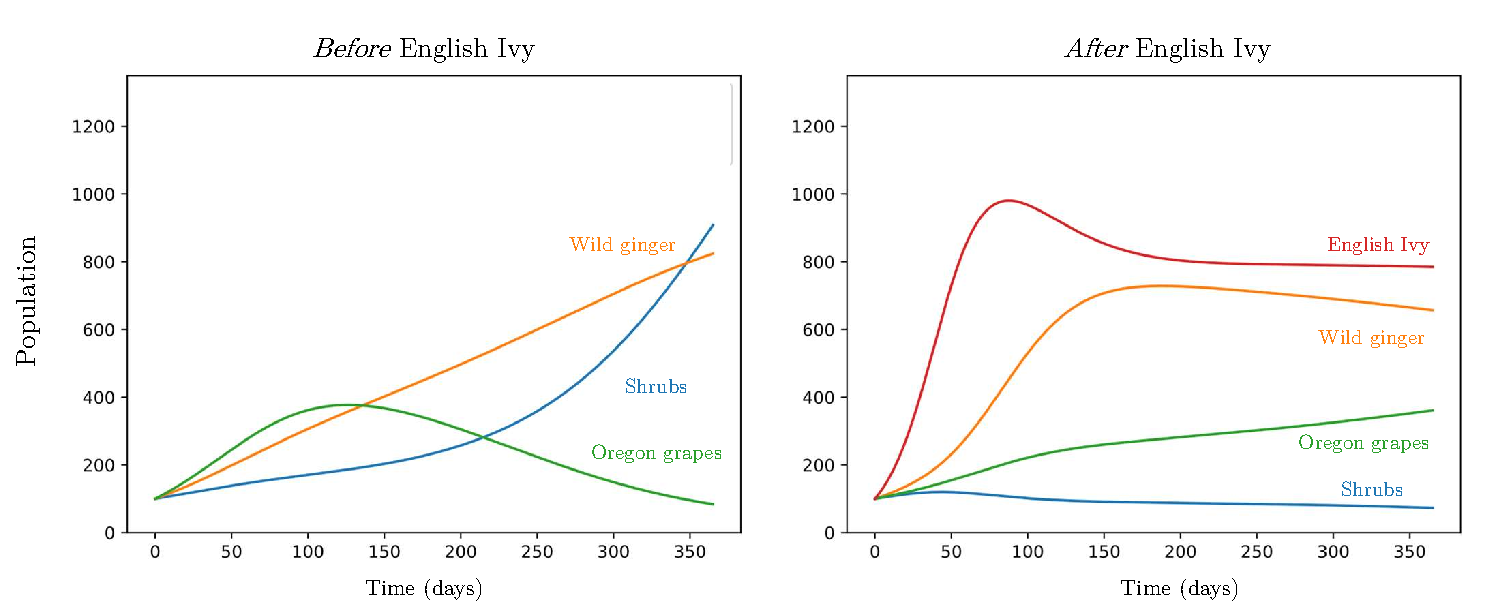
\includegraphics[scale=0.5]{figures/lotkavolterraenglishivy.pdf}
    \captionsetup{width=0.9\textwidth}
    \caption{\textbf{Before and after plot of native species populations of introduction of English ivy species.}}
    \label{fig:lotkavolterraenglishivy}
\end{figure}

From graphing the population solutions to the system, we can see the population shifts in Figure~\ref{fig:lotkavolterraenglishivy}. Based on the numerical solution to this differential equation from scientific computing software, we find the change of populations over a single year (365 days) to be \(\frac{900}{90}\) for shrubs, \(\frac{800}{600}\) for wild ginger, and \(\frac{100}{300}\) for Oregon grapes. So, we can calculate the native species impact score to be

\[\chi = \frac{900}{90} + \frac{800}{600} + \frac{100}{300} = 11.667\]

For the second part of the ecological score, we need to calculate the spreadability index. First, we can start from a commonly regarded fact that English populations can double in around one and a half years in most growing conditions, even in the shade \cite{usdaHederaHelix}. Therefore, by performing logistic regression with the x-axis being days and the y-axis as population, we can find that the \(r\) value is around 0.035. So, our spreadability index can be calculated as \(100r = 3.5\). Therefore, by Equation~\ref{eq:ecologicalimpact}, our ecological impact score is \(3.5 + \chi = 3.5 + 11.667 = 15.167\).

\subsubsection{Economic Potential}
We assume that there exists some small landscaping firm which harvests and grows English ivy plants in a town in Washington, as common landscaping designers use English ivy to decorate their clients' backyards \cite{psuEnglishLandscape}. By analyzing the microeconomic model of this firm, we will be able to calculate our economic profits.

First, we start with estimating the expected marginal cost and revenue of harvesting and growing each pound of English ivy based on the Gordon-Schaefer model. We estimate that the constant marginal cost of harvesting each pound of English ivy is around \(\$15.00\), as in a larger operation, it takes around an hour of manual labor to safely harvest English ivy \cite{bhgCaringEasytoGrow}. 

To estimate marginal revenue, we performed an online survey to estimate revenue per pound of English ivy. Based on several pricing estimates \cite{gardengoodsdirectEnglish}, we conclude that the maximum pricing for a pound of English ivy would fall around \(\$100.00\) and decreasing with slope \(-0.5\) per pound increased of English ivy. After applying the Profit Maximization Law and analyzing this firm like a Gordon-Schaefer model and finding the intersection of the MR and MC curve, it is evident that an optimal English ivy yield would be around 170 lbs for \(\$57.75\) each. 

To calculate economic profits (\(\pi\)), we subtract total costs (\(\$15.00 \cdot 170\)) from total revenue (\(\$57.75 \cdot 170\)), which leads us to conclude that \(\pi = \$7225.00\).

As for measuring social welfare, English ivy has no benefits to humans other than as a landscaping plant, which is already a core part of calculating economic profits. Lastly, for the human risk factor, English ivy is inedible and contains toxic sap, however, there is rarely an incidence where an English ivy plant has harmed a human. Therefore, we deduce that social welfare \(W = 0\) and human risk \(R = 0\). So, our total economic potential can be calculated as 

\[\text{Total Economic Benefit } = \pi + W - R = \$7225.00\]

So, our final invasive species impact score for English ivy plants in Washington is

\[\text{Impact Score} = (\text{Ecological Score, Economic Score}) = (15.167, \$7225.00)\]

\subsection{Score Comparison}

To analyze the differences in each score and the "classification" of each non-native species, we take a look at the trade-offs between ecological and economic scores in our definition of an impact factor.

\begin{table}[h]
\renewcommand{\arraystretch}{1.3}
%p{0.8\linewidth
    \begin{tabularx}{\textwidth}{p{0.21\textwidth}llX}
    \toprule
    \textbf{Non-Native Species}  & \textbf{Ecological} & \textbf{Economic} & \textbf{Analysis} \\ \midrule
    \raggedright Dandelions & 21.794 & \(\$105.46\) & As dandelions have a high ecological impact primarily due to the loss of native populations with a low return in economic potential, we conclude that dandelions are indeed \textit{invasive species}. \\
    \rowcolor{gray!15}
    \raggedright Garlic mustard & 5.278  & \(\$26.00\) & Since garlic mustard plants have a slight ecological impact and have little to none return on economic potential, we label garlic mustard plants as \textit{invasive species.}\\
    \raggedright English ivy & 15.167 & \(\$7225.00\) & As English ivy plants have a high impact on environment yet also have a large return on economic potential, we conclude that English ivy plants \textit{are not invasive}.\\
    \bottomrule
    \end{tabularx}
\end{table}

\section{Invasive Species Trade-Off Model Discussion}

\subsection{Model Generalization}

When applying our model to a larger sample of foreign plants to classify them as invasive or not invasive, it would be immensely beneficial to create an auto-classification system. Such a classification system would consist of a "line of division" in a plot where each axis would represent the ecological or economic scores. Since we do not have enough data points to create such a classification system, we design a \textit{DSD} framework (Data-Score-Divide) below where an environmental scientist may use our trade-off model.

In our proposed \textit{DSD} framework, environmental scientists would perform the following steps as described in Figure~\ref{fig:dsdprocess}. First, a scientist must collect regional native population data, economic costs and revenues from similar firms, and determine dollar-value human risk costs in local populations. Next, data is to be evaluated via our proposed ecological and economic scores. Finally, scores for each foreign species should be plotted on an economic versus ecological score plot, where a line of division must be drawn by an evaluator to specify the split between invasive and simply foreign species. This division process is inspired by Support Vector Machines, which are commonly used in machine learning classification tasks \cite{ieeeSupportVector}.

We did not conduct a sensitivity analysis on our trade-off model because, in a sense, the environmental scientists who \textit{divide} the scores are the primary influences of the final decision.

\begin{figure}[h!]
\centering
    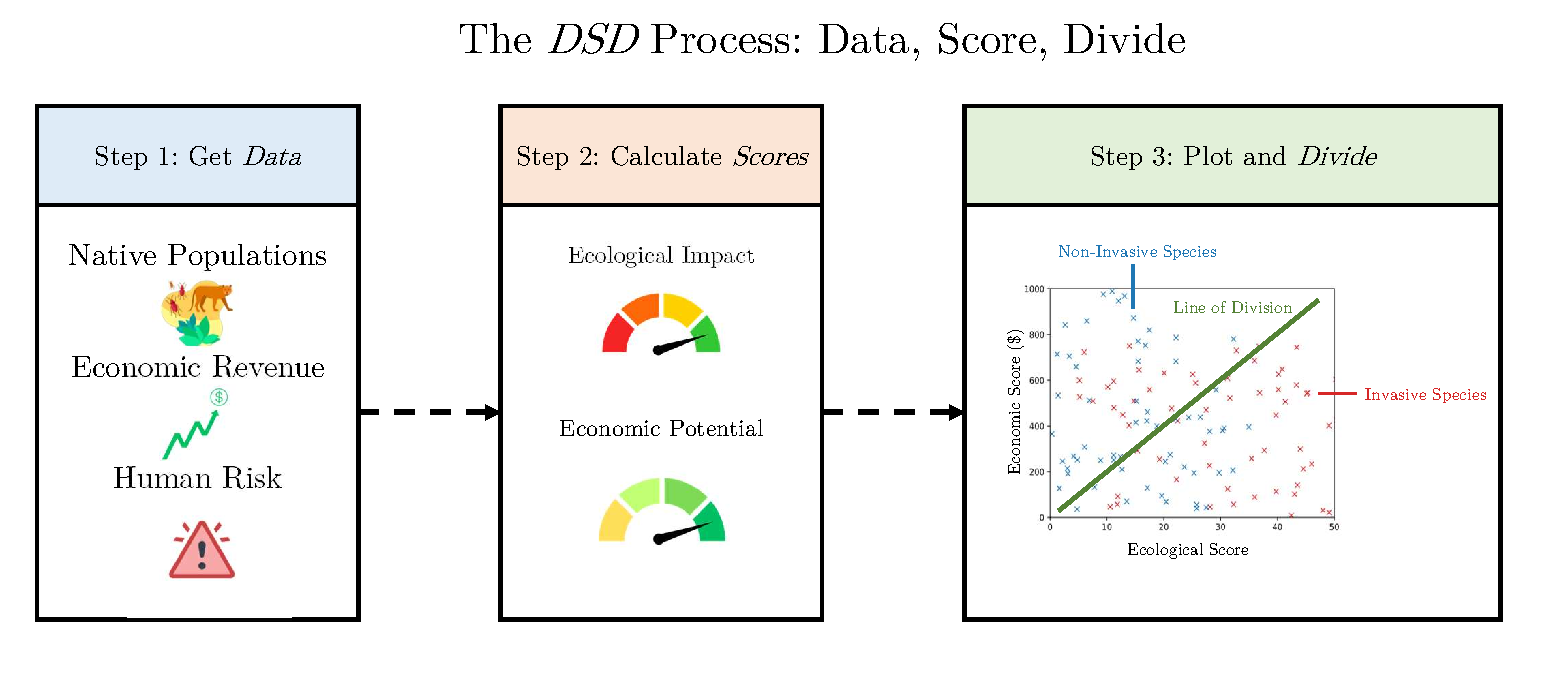
\includegraphics[scale=0.6]{figures/dsdprocess.pdf}
    \captionsetup{width=0.9\textwidth}
    \caption{\textbf{The \textit{Data-Score-Divide} (DSD) framework for evaluating foreign species.}}
    \label{fig:dsdprocess}
\end{figure}

\subsection{Strengths}
\begin{enumerate}
    \item Our model offers unique\textbf{ insights into the trade-offs} of foreign species, in particular, invasive species.
    \begin{quote}
        Unlike impact models that only examine the ecological benefits and downfalls of a foreign species, our model examines both ecological and economic trade-offs.
    \end{quote}
    \item Our model is adaptable to virtually \textbf{any region and foreign plant} combination.
    \begin{quote}
        This means that our model can be applied to different scenarios and contexts, such as invasive species management, biodiversity conservation, and ecological restoration. Our model can adapt based on different regional native plants and economic conditions. We also provide a general-use framework that can be quickly applied to many species at a time.
    \end{quote}
\end{enumerate}
\subsection{Limitations}
\begin{enumerate}
\item Intra-population dynamics between foreign and native species that are unknown \textbf{can be difficult to predict}.
    \begin{quote}
     In the previous three contexts of analyzing the trade-offs between dandelion, garlic mustard, and English ivy plants, the most distinct aspect of these species is that they are widely classified as invasive or a "weed." This means that for unknown foreign species relationships, scientists must input some observational data into the model.
    \end{quote}
\item New economic benefits and pitfalls \textbf{may not follow historical trends}.
\begin{quote}
    In our analysis of dandelion and English ivy plants, several businesses centered around dandelion and English ivy harvesting already exist. This allows us to build upon previous work to calculate new economic profits and yield. However, when we take a look at the case of garlic mustard plants, few garlic mustard firms exist, which hinders our ability to predict economic outcomes.
\end{quote}
    
\end{enumerate}



%%%%%%%%%%%%%%%%%%%%%

\section{Conclusion}
In this paper, we developed a mathematical model to predict the spread of dandelions and evaluate whether they are genuinely invasive. Our seed agent model considers the different phases of a dandelion's life cycle, including seed dispersal, germination, plant development, and the puffball stage. The model also considers environmental factors such as temperature, light, and nutrients. The paper discusses the application of the model to three different regions and analyzes the ecological impact and economic potential of other invasive species.

To evaluate foreign species' trade-offs, we formulate an impact score based on ecological and economic factors. Furthermore, our model is adaptable as we provide a unique framework for different regions and foreign plant combinations. 

\newpage

\bibliographystyle{abbrv}

{\scriptsize
\bibliography{HiMCM}
}

\pagebreak

\section{Appendices}
\subsection{Appendix 1: Seed Agent Modeling Code}
\insertcode{./seedagentmodel.py}{code/main.py}


\end{document}


